\documentclass[final]{fhnwreport}       %[mode] = draft or final
                                        %{class} = fhnwreport, article, 
                                        %          report, book, beamer, standalone
%%---Main Packages-----------------------------------------------------------------------
\usepackage[english, ngerman]{babel}	%Mul­tilin­gual sup­port for LaTeX
\usepackage[T1]{fontenc}				%Stan­dard pack­age for se­lect­ing font en­cod­ings
\usepackage[utf8]{inputenc}				%Ac­cept dif­fer­ent in­put en­cod­ings
\usepackage{lmodern}                    %The newer Font-Set
\usepackage{textcomp}					%LaTeX sup­port for the Text Com­pan­ion fonts
\usepackage{graphicx} 					%En­hanced sup­port for graph­ics
\usepackage{float}						%Im­proved in­ter­face for float­ing ob­jects
\usepackage{ifdraft}                    %Let you check if the doc is in draft mode

%%---Useful Packages---------------------------------------------------------------------
\usepackage[pdftex,dvipsnames,table]{xcolor}  %Driver-in­de­pen­dent color ex­ten­sions for LaTeX
\usepackage{csquotes}                   %Simpler quoting with \enquote{}
\usepackage{siunitx} 					%A com­pre­hen­sive (SI) units pack­age
\usepackage{listings}					%Type­set source code list­ings us­ing LaTeX
\usepackage[bottom]{footmisc}			%A range of foot­note op­tions
\usepackage{footnote}					%Im­prove on LaTeX's foot­note han­dling
\usepackage{verbatim}					%Reim­ple­men­ta­tion of and ex­ten­sions to LaTeX ver­ba­tim
\usepackage[textsize=footnotesize]{todonotes} %Mark­ing things to do in a LaTeX doc­u­ment
\usepackage{booktabs}
\usepackage{lscape}
\usepackage{blindtext}
\usepackage{wrapfig}
\usepackage{caption}
\usepackage{romannum}

%%---Tikz Packages-----------------------------------------------------------------------
\usepackage{standalone}
\usepackage{tikz}
\usepackage{circuitikz}
\usetikzlibrary{arrows}
\usetikzlibrary{calc}
\usetikzlibrary{intersections}

%%---Math Packages-----------------------------------------------------------------------
\usepackage{amsmath}					%AMS math­e­mat­i­cal fa­cil­i­ties for LaTeX
%\usepackage{amssymb}					%Type­set­ting symbols (AMS style)
%\usepackage{array}						%Ex­tend­ing the ar­ray and tab­u­lar en­vi­ron­ments
%\usepackage{amsthm}					%Type­set­ting the­o­rems (AMS style)

%%---Table Packages----------------------------------------------------------------------
\usepackage{tabularx}					%Tab­u­lars with ad­justable-width columns
%\usepackage{longtable}
\usepackage{multirow}					%Create tab­u­lar cells span­ning mul­ti­ple rows
\usepackage{multicol}					%In­ter­mix sin­gle and mul­ti­ple columns

%%---PDF / Figure Packages---------------------------------------------------------------
\usepackage{pdfpages}					%In­clude PDF doc­u­ments in LaTeX
\usepackage{pdflscape}					%Make land­scape pages dis­play as land­scape
\usepackage{subfig}					    %Fig­ures di­vided into sub­fig­ures

%%---Other Packages----------------------------------------------------------------------
%\usepackage{xargs}                     %De­fine com­mands with many op­tional ar­gu­ments

%%---Bibliography------------------------------------------------------------------------
\usepackage[style=ieee,urldate=comp,backend=biber]{biblatex}
\addbibresource{literature/bibliography.bib}

%%---Main Settings-----------------------------------------------------------------------
\graphicspath{{./graphics/}}			%Defines the graphicspath
%\geometry{twoside=false}				    %twoside=false disables the "bookstyle"
\setlength{\marginparwidth}{2cm}
\overfullrule=5em						%Creates a black rule if text goes over the margins => debugging


%%---User Definitions--------------------------------------------------------------------
%%Tabel-Definitions: (requires \usepackage{tabularx})
\newcolumntype{L}[1]{>{\raggedright\arraybackslash}p{#1}}    %column-width and alignment
\newcolumntype{C}[1]{>{\centering\arraybackslash}p{#1}}
\newcolumntype{R}[1]{>{\raggedleft\arraybackslash}p{#1}}

%%---Optional Package Settings-----------------------------------------------------------
%Listings-Settings: (requires \usepackage{listings}) => Example with Matlab Code
\lstset{language=Matlab,%
    basicstyle=\footnotesize\ttfamily,
    breaklines=false,%
    morekeywords={switch, case, otherwise},
    keywordstyle=\color{Blue},%
    tabsize=2,
    %morekeywords=[2]{1}, keywordstyle=[2]{\color{black}},
    identifierstyle=\color{Black},%
    stringstyle=\color{Purple},
    commentstyle=\color{Green},%
    showstringspaces=false,%without this there will be a symbol in the places where there is a space
    numbers=left,%
    numberstyle={\tiny \color{black}},% size of the numbers
    numbersep=9pt, % this defines how far the numbers are from the text
    %emph=[1]{word1, word2,...},emphstyle=[1]\color{red}
}					

			                %loads all packages, definitions and settings	

									
\title{\Huge{\textbf{Wetterstation mit Solar Energie}}\\}          %Project Title
\author{\huge{Bachelor Diplomarbeit 2019}}          %Document Type => Technical Report, ...
\date{Brugg/Windisch, \today}             %Place and Date


\begin{document}

%%---TITLEPAGE---------------------------------------------------------------------------
\selectlanguage{ngerman}                %ngerman or english
\maketitle
%\vspace*{-1cm}
\vspace*{-0.5cm}						    %compensates the space after the date line.
\vfill
\begin{figure}[H]
\centering
%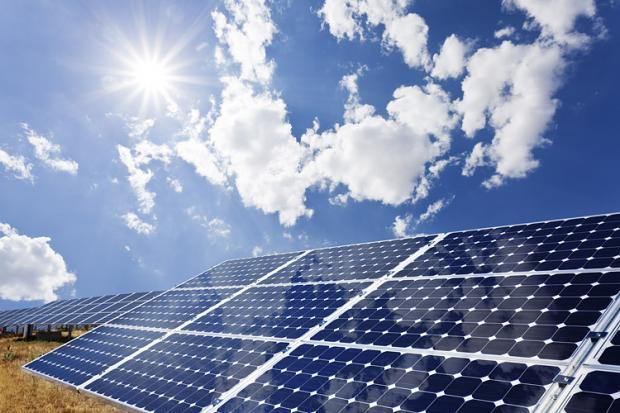
\includegraphics[width=\linewidth]{Titelbild.jpg}
\end{figure}
\vfill

{
\renewcommand\arraystretch{2}
\begin{center}
\begin{tabular}{p{4cm} l}
\textbf{Hochschule}				&    Hochschule für Technik - FHNW\\
\textbf{Studiengang}			&    Elektro- und Informationstechnik\\
\textbf{Autoren}				& 	Mischa Knupfer, Andres Minder\\
\textbf{Auftraggeber}			&    Prof. Dr. Taoufik Nouri\\
\textbf{Experte}				&	Patrick Strittmatter\\
\textbf{Betreuer}				&    Prof. Dr. Taoufik Nouri\\
\textbf{Version}				&    2.1 %Normally not used!
\end{tabular}
\end{center}
}

\clearpage
			
%%---ABSTRACT----------------------------------------------------------------------------
\selectlanguage{english}				%ngerman or english
\thispagestyle{empty}
\pagenumbering{Roman}
\begin{abstract}
\noindent
Climate and weather data are the main sources to determine plots for specific plants or plant species for a specific climate. Because of that, farmers need to know the climate and weather data to optimize their work. Swiss farmers have the advantage of getting this information through a federal agency, which does not apply to farmers in subtropical areas. To provide these information for farmers in subtropical areas, a low-priced mobile weather station is required. This project should design a prototype of a weather station, which can record data for air temperature, Rainfall, wind strength and hours of sunshine. In addition to that, the DS3231 real time clock (RTC) should generate a timestamp to the data before it is stored in the data memory. The core of the weather station is the microcontroller ArduinoMega2560, which contains the program code and manages the data storage. The wind strength is being measured by the WD123 from Froggit, the rainfall by an ombrometer from Misol and the air temperature by the BME280 from Bosch that measures also humidity and pressure of the air. Moreover, a wind vane (p/n 80422) from Argent Data Systems allows the weather station to determine the wind direction. Those gained data points are stored on an internal microSD card.\\[0.5cm]
The mobile weather station is able to provide data for temperature, humidity and pressure of the air as well as the Rainfall and the strength and direction of the wind. Furthermore, the mobile weather station is also able to store the data points with timestamp on the microSD card. In a further project, a battery will be implemented which will be supported by photovoltaic. Furthermore, GPS and data query over SMS (GSM) will also be implemented in that further project.\\
\\
Key Words: mobile weather station, sensors, microSD card, GPS, SMS (GSM)


\end{abstract}	

%%---TABLE OF CONTENTS-------------------------------------------------------------------
\selectlanguage{ngerman}				%ngerman or english
\tableofcontents
\clearpage

%%---TEXT--------------------------------------------------------------------------------
\pagenumbering{arabic}

\part{Einleitung}
\label{part:EinleitenderTeil}
\chapter{Einleitung}
\label{chap:Einleitung}
\chapter{Auftragsbeschreibung}
\label{chap:Auftrag}
\chapter{Ziele}
\label{chap:Ziele}
\chapter{Konzept}
\label{chap:Konzept}

\part{Firmware}
\label{part:Firmware}
\chapter{Interfaces}
\label{chap:Interfaces}
\chapter{Firmware}
\label{chap:Firmware}

\part{Hardware}
\label{chap:Hardware}
\chapter{Übersicht}
\label{chap:Uebersicht}
\chapter{MCU}
\label{chap:MCU}
Im Projekt 5 wurde bereits eine MCU ausgewählt, mit der das Prototyping erfolgte. Aufgrund der Verfügbarkeit (bei der FHNW bezugsbereit) wurde ein Arduino Mega2560 Board verwendet. Auf den kommenden Abschnitt aus dem Fachbericht des Projekt 5 folgt ein Abschnitt mit ergänzenden Informationen aus der Bachelor-Thesis.

\section{MCU - Projekt 5}
Die Micro Controller Unit (MCU) ist der zentrale Bestandteil für die Kommunikation, resp. für den Datenaustausch zwischen den unterschiedlichen Modulen. Sie interpretiert die Signale der Sensoren und rechnet sie in die interessierenden Messwerte um. Dann weist die MCU jedem Messwert einen Zeitstempel über das RTC zu und übergibt diesen der Datenspeicherung. Wenn die Daten vom Kommunikationsmodul angefordert werden, liest die MCU die Datenspeicherung aus und übergibt sie dem Kommunikationsmodul.\\

{\begin{minipage}[b][130pt][t]{0.5\textwidth}
Für die Entwicklung der MCU wird ein Arduino Mega Board verwendet. Der Vorteil besteht darin, dass elementare Bauteile (Hardware) bereits implementiert sind, wie z.B. Oszillator, der USB-Anschluss und die PCB-Connectors für ein schnelles Prototyping. Die wichtigsten technischen Daten sind in der Tabelle \ref{tab:arduinoMega_technischeDaten} aufgelistet.\\
\end{minipage}}
\hfill
{\begin{minipage}[b][130pt][t]{0.49\textwidth}
\centering
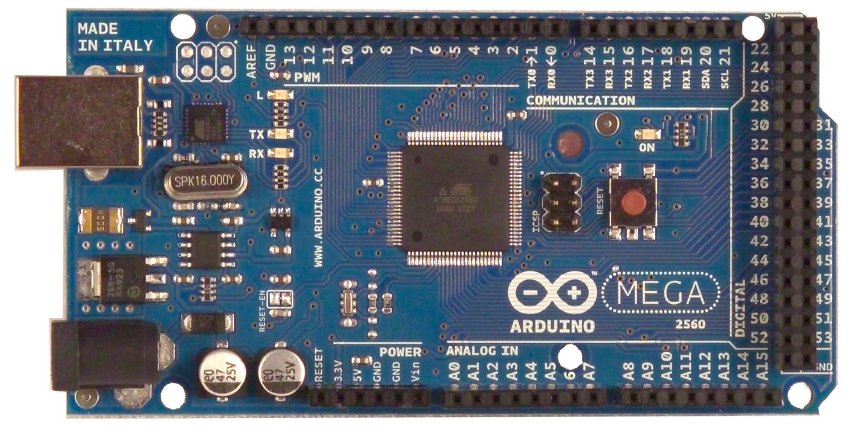
\includegraphics[width=0.99\textwidth]{graphics/MCU/arduino_mega.png}
\captionof{figure}{Arduino Mega Board \cite[S.1]{arduinoMega}}
\label{fig:arduinoMega}
\end{minipage}}

\begin{table}[h]
\centering
\caption{Technische Daten \cite[S.3]{arduinoMega}}
\begin{tabular}{|l|l|}
\hline 
Microcontroller & ATmega2560 \\ 
\hline 
Operating Voltage & 5V \\ 
\hline 
Digital I/O Pins & 54  \\ 
\hline 
Analog Input Pins & 16 \\ 
\hline 
Flash Memory & 256 KB, 8 KB werden vom bootloader benötigt\\ 
\hline 
SRAM & 8 KB \\ 
\hline 
EEPROM & 4 KB \\ 
\hline 
Clock Speed & 16 MHz \\ 
\hline 
\end{tabular}
\label{tab:arduinoMega_technischeDaten}
\end{table}

\section{Ergänzungen aus der Bachelor-Thesis}
Während der Bachelor-Thesis kam die Idee auf, eine kleinere MCU zu verwenden. Eine kleinere MCU hat die Vorteile, dass diese günstiger ist in der Anschaffung, einen geringeren Stromverbrauch aufweist und weniger Platz auf dem PCB benötigt.  Aufgrund der Firmware wird jedoch eine erhöhte Menge Speicher alloziert, weshalb die \textit{Data Memory Usage} des verwendeten ATMega328 zu klein war und wieder auf den bereits für das Prototyping verwendeten ATMega2560 zurückgegriffen werden musste. \\

\chapter{RTC}
\label{chap:RTC}
\chapter{Sensoren}
\label{chap:Sensoren}
Der grossteil der Sensorik wurde bereits während des Projekt 5 implementiert und in dessen Fachbericht dokumentiert. Die Dokumentation der bereits implementierten Sensoren wird in nachfolgendem Abschnitt inkludiert und darauf folgend der Sensor zur Messung der Sonnenstunden, welcher während der Bachelor-Thesis imeplementiert wurde, in einem separaten Abschnitt erläutert.\\

\section{Sensoren - Projekt 5}
\subsection{Ombrometer}

\subsubsection*{Ermittlung der Niederschlagsmenge}
Dieses Unterkapitel befasst sich mit der Realisierung der Niederschlagsmessung. Diese soll nach einem Kipplöffelprinzip funktionieren und gemäss definierten Zielen eine Genauigkeit von $\pm$100 ml/$m^2$ aufweisen. Ausserdem soll als alternative zusätzlich ein Messbecher an der Wetterstation installiert werden, damit der Bauer die Niederschlagsmenge anhand einer Skala ablesen kann. In einem ersten Schritt soll das Kipplöffelprinzip näher erläutert und mit einem Selbstbau die Funktionsweise getestet werden. Anschliessend soll ein gekaufter Sensor die Wetterstation erweitern und die Implementation in der Firmware thematisiert werden. Zu guter Letzt soll die Validierung des Teilsystems folgen.
\subsubsection*{Das Kipplöffelprinzip}
Das Prinzip des Kipplöffels wird in Abbildung \ref{fig:Kipp} graphisch dargestellt.

\begin{figure}[h]
\centering
\includegraphics[width=0.8\linewidth]{graphics/Kipploeffel.png}
\caption{Darstellung des Kipplöffelprinzips}
\label{fig:Kipp}
\end{figure}

Abbildung \ref{fig:Kipp} zeigt das Kipplöffelprinzip. Der Kipplöffel (\glqq 3)\grqq) besteht im Grunde aus zwei Löffeln und ist in der Mitte drehbar mit dem Gehäuse befestigt (\glqq 4)\grqq). Regenwasser wird über eine Öffnung im Gehäusedeckel (Trichter, \glqq 1)\grqq) zum Kipplöffel befördert (\glqq 2)\grqq). Ist der Löffel mit Regenwasser gefüllt, so kippt dieser aufgrund des Gewichts und leert das Wasser über eine Öffnung im Gehäuseboden (\glqq 5)\grqq) aus. Durch die Kippung wird der andere Löffel in die Ausgangsposition bewegt und kann sich nun mit Wasser füllen. Mit der Hilfe von Reedkontakten und Magneten wird die Anzahl der Kippbewegungen gezählt. Die Niederschlagsmenge ergibt sich aus der Anzahl Kippbewegungen, multipliziert mit dem Volumen des Kipplöffels.
\newpage

\subsubsection*{Die Realisierung des Niederschlagsmengensensors}
Um die Funktionsweise des Niederschlagsmengensensors  zu testen, wird, wie im Pflichtenheft festgehalten, dieser in einem ersten Schritt selbst erstellt. Die Erstellung kann in vier Etappen unterteilt werden. Die erste Etappe ist die Erstellung des Kipplöffels. Die zweite Etappe folgt mit der Erstellung der Drehbaren Lagerung. Als dritte Etappe folgt der Trichter und die vierte und letzte Etappe widmet sich dem Gehäuse, wobei der Trichter ein Teil des Gehäuses darstellt. Das Gehäuse wird, bei verwendung der Eigenproduktion, erst im Projekt 6 mit dem Gehäuse der gesamten Wetterstation erstellt.
\paragraph{Etappe 1: Realisierung des Kipplöffels}
Wichtig für die Erstellung des Kipplöffels sind die Dimensionierung und die Materialwahl.
 
Das Material soll wetterbeständig, einfach bearbeitbar und günstig sein und eine möglichst glatte Oberfläche haben. Die möglichst glatte Oberfläche ist notwendig, damit das Wasser im Kipplöffel sich nicht an der Oberfläche festhält und somit gut abfliesst. Acrylglas erfüllt diese Bedingungen und ist in jedem Baumarkt erhältlich, weshalb es als Material gewählt wird.

Die Dimensionierung ist Abhängig von der gewählten Genauigkeit im Pflichtenheft. Damit eine Genauigkeit von $\pm$100 ml/$m^2$ erreicht werden kann, müssen beide Löffel des Kipplöffels bei genau 100 ml Fassungsvermögen kippen. Damit dies erreicht wird, kann man physikalisch die statische Gleichgewichtsbedingung aufstellen und daraus die Dimensionierung folgern. Dies ist jedoch ein sehr aufwändiger, komplizierter und zeitintensiver weg. Einfacher ist es, wenn der Kipplöffel extra zu gross dimensioniert und die Füllmenge im nachhinein justiert wird. Die Justierung erfolgt mittels einer in der Höhe verstellbaren Lagerung, sowie mit in der Höhe verstellbaren Schrauben im Gehäuseboden, welche die Neigung der Endposition des Kipplöffels beeinflusst. Ein weiterer Vorteil dieser Nachjustierung ist, dass auch eine andere Füllmenge einstellbar wäre.

\begin{figure}[h]
\centering
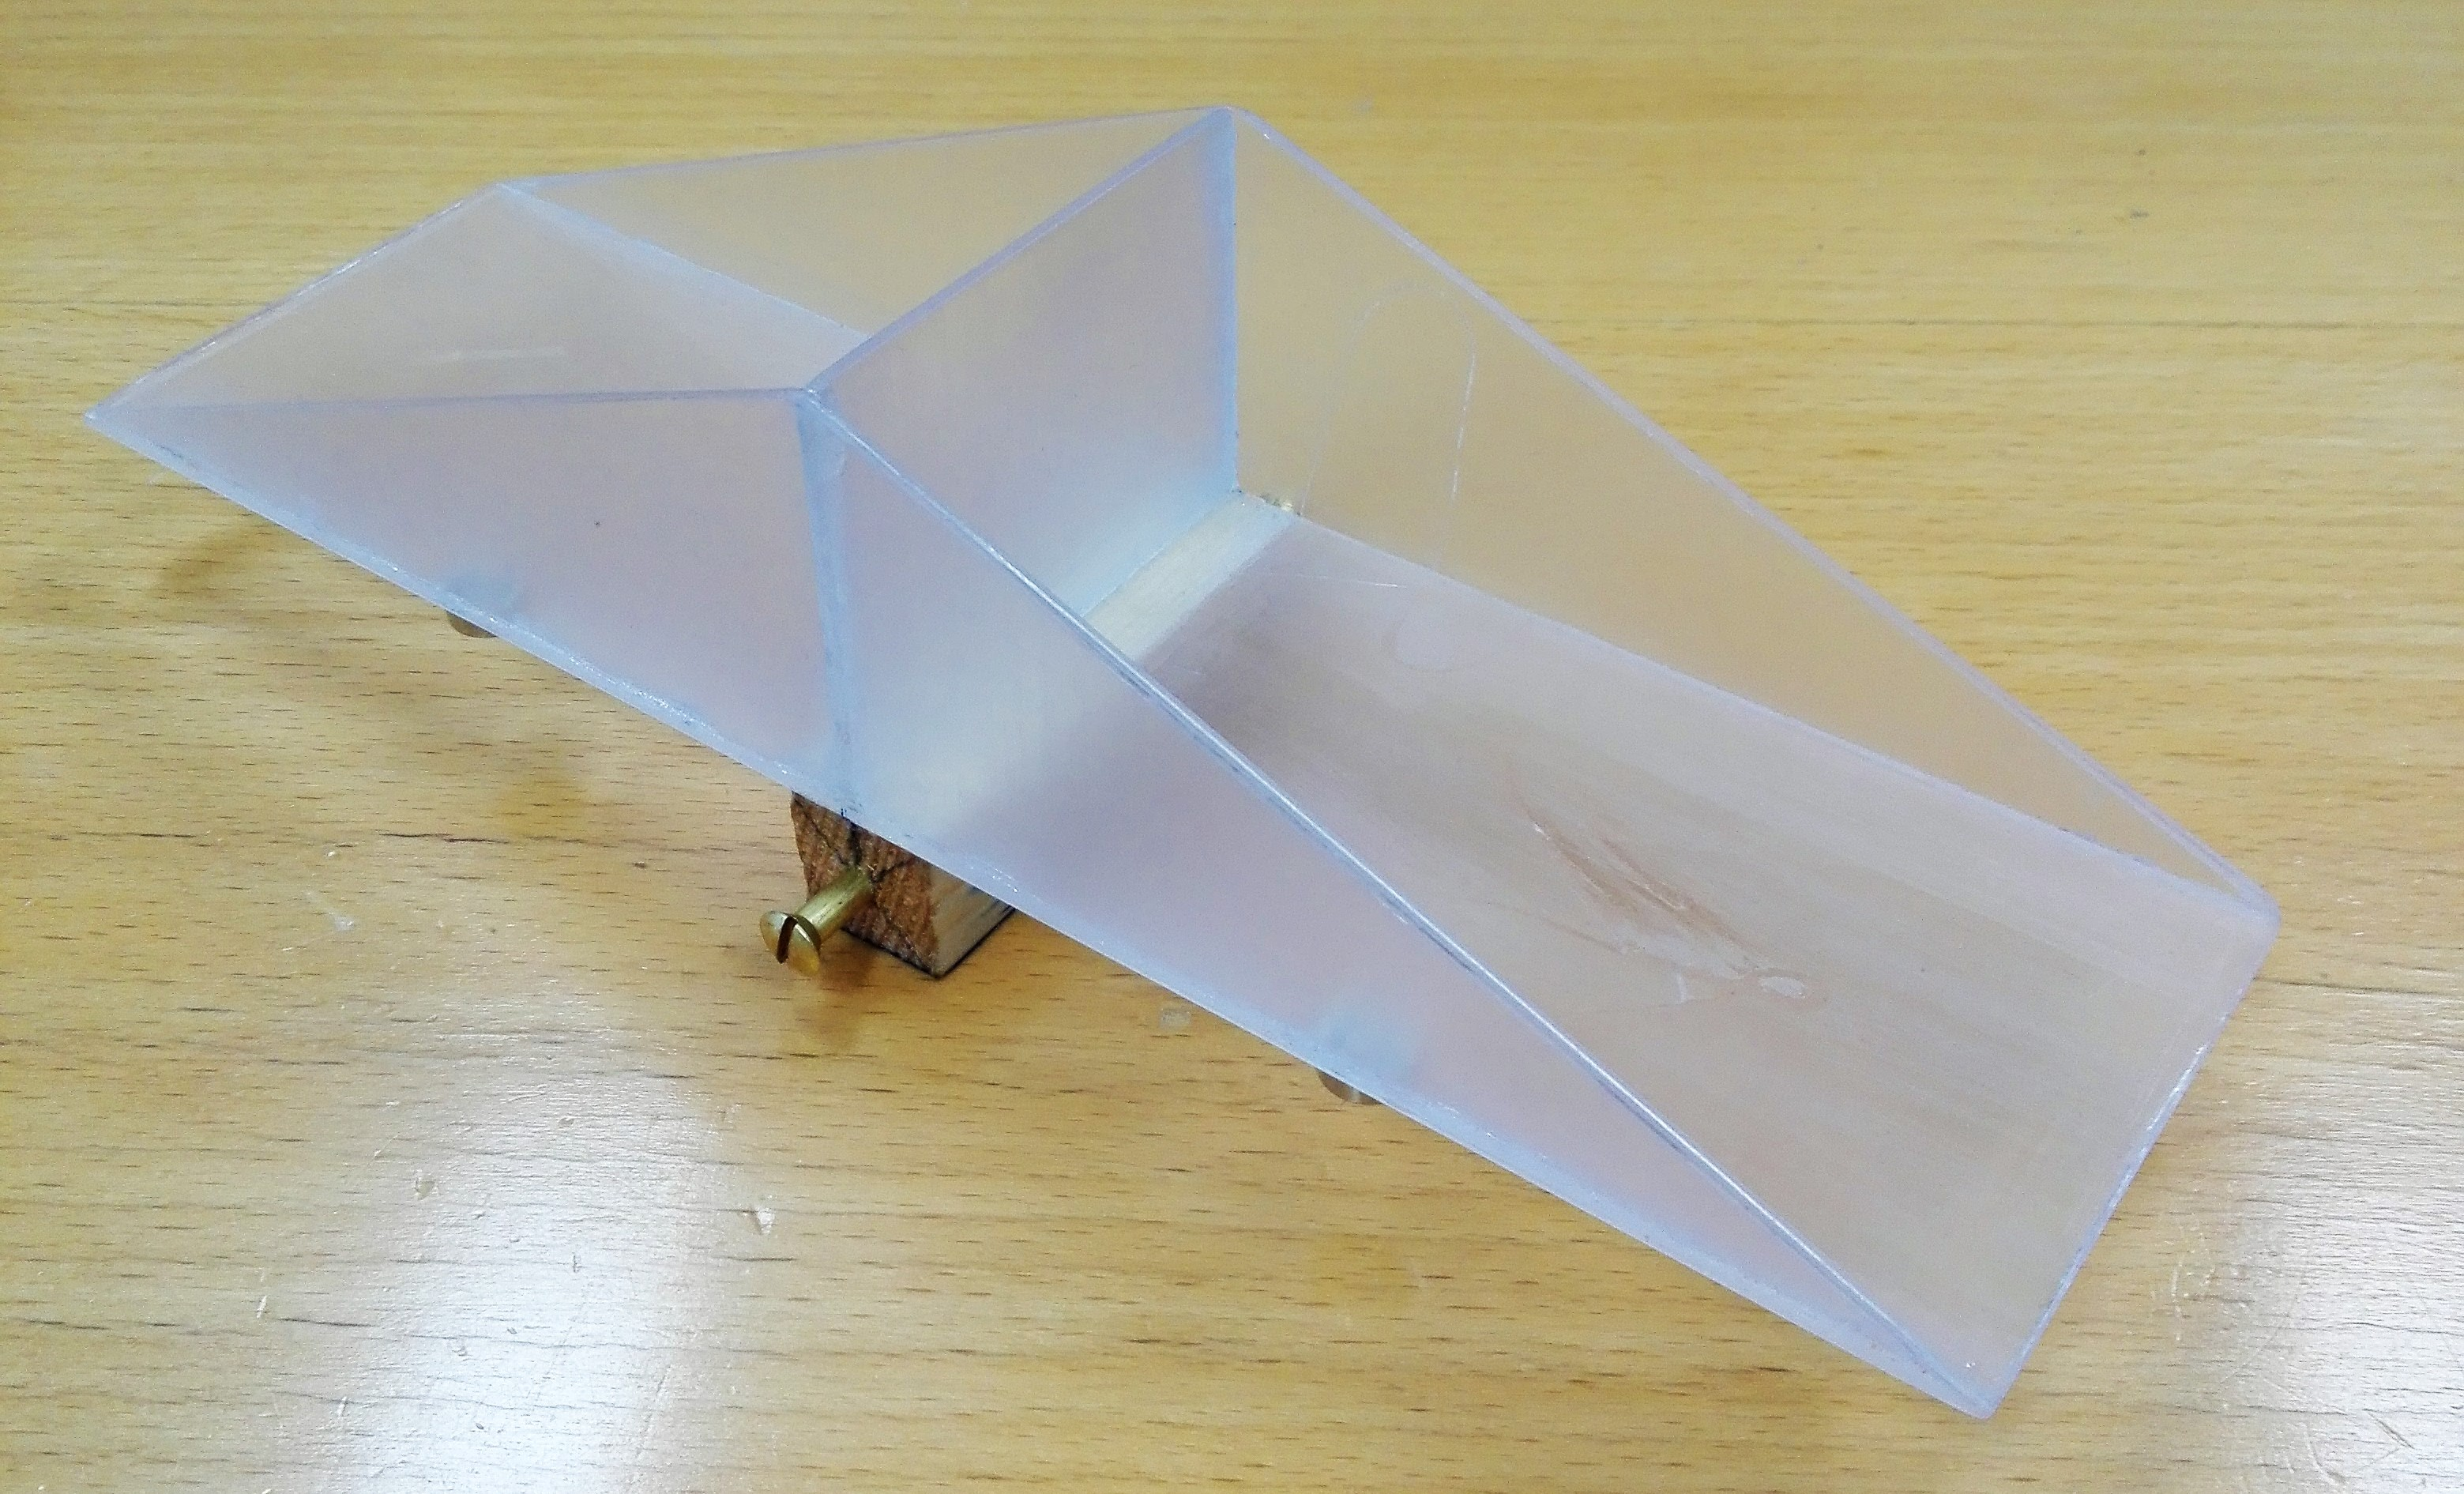
\includegraphics[width=0.8\linewidth]{graphics/Etappe1.jpg}
\caption{Selbsterstellter Kipplöffel.}
\label{fig:Etappe1}
\end{figure}

Abbildung \ref{fig:Etappe1} zeigt den selbsterstellten Kipplöffel aus Acrylglas. Die Drehachse ist mittig unter dem Kipplöffel befestigt und besteht aus einem Holzklotz mit je einer Schraube pro Seite.

\paragraph{Etappe 2: Realisierung der drehbaren Lagerung}
Die Drehbare Lagerung des Kipplöffels ist wichtig, damit der Kipplöffel auf beide Seiten kippen kann. Die Drehachse soll direkt unterhalb der Mitte des Kipplöffels befestigt sein um ein gleichmässiges Kippen zu ermöglichen. Die Höhe des Kipplöffels wird definiert durch die einstellbare Höhe der Drehachsenlagerung. 

Die Drehachse wird aus einem Stück Holz und zwei Schrauben gefertigt, wobei das Holz direkt am Kipplöffel befestigt wird. Die zwei Schrauben werden auf einem höhenverstellbarem Gerüst gelagert, so dass ein drehen möglich ist. Dieses Gerüst wird auch aus Holz gefertigt und enthält eine Metallische Fläche an der Kontaktstelle der zuvor erwähnten Schrauben, um aufkommende Reibkräfte zu verringern. Ausserdem ist dieses Gerüst höhenverstellbar über zwei mit Muttern feststellbaren Gewinden (für jede Seite eine). 

\begin{figure}[h]
\centering
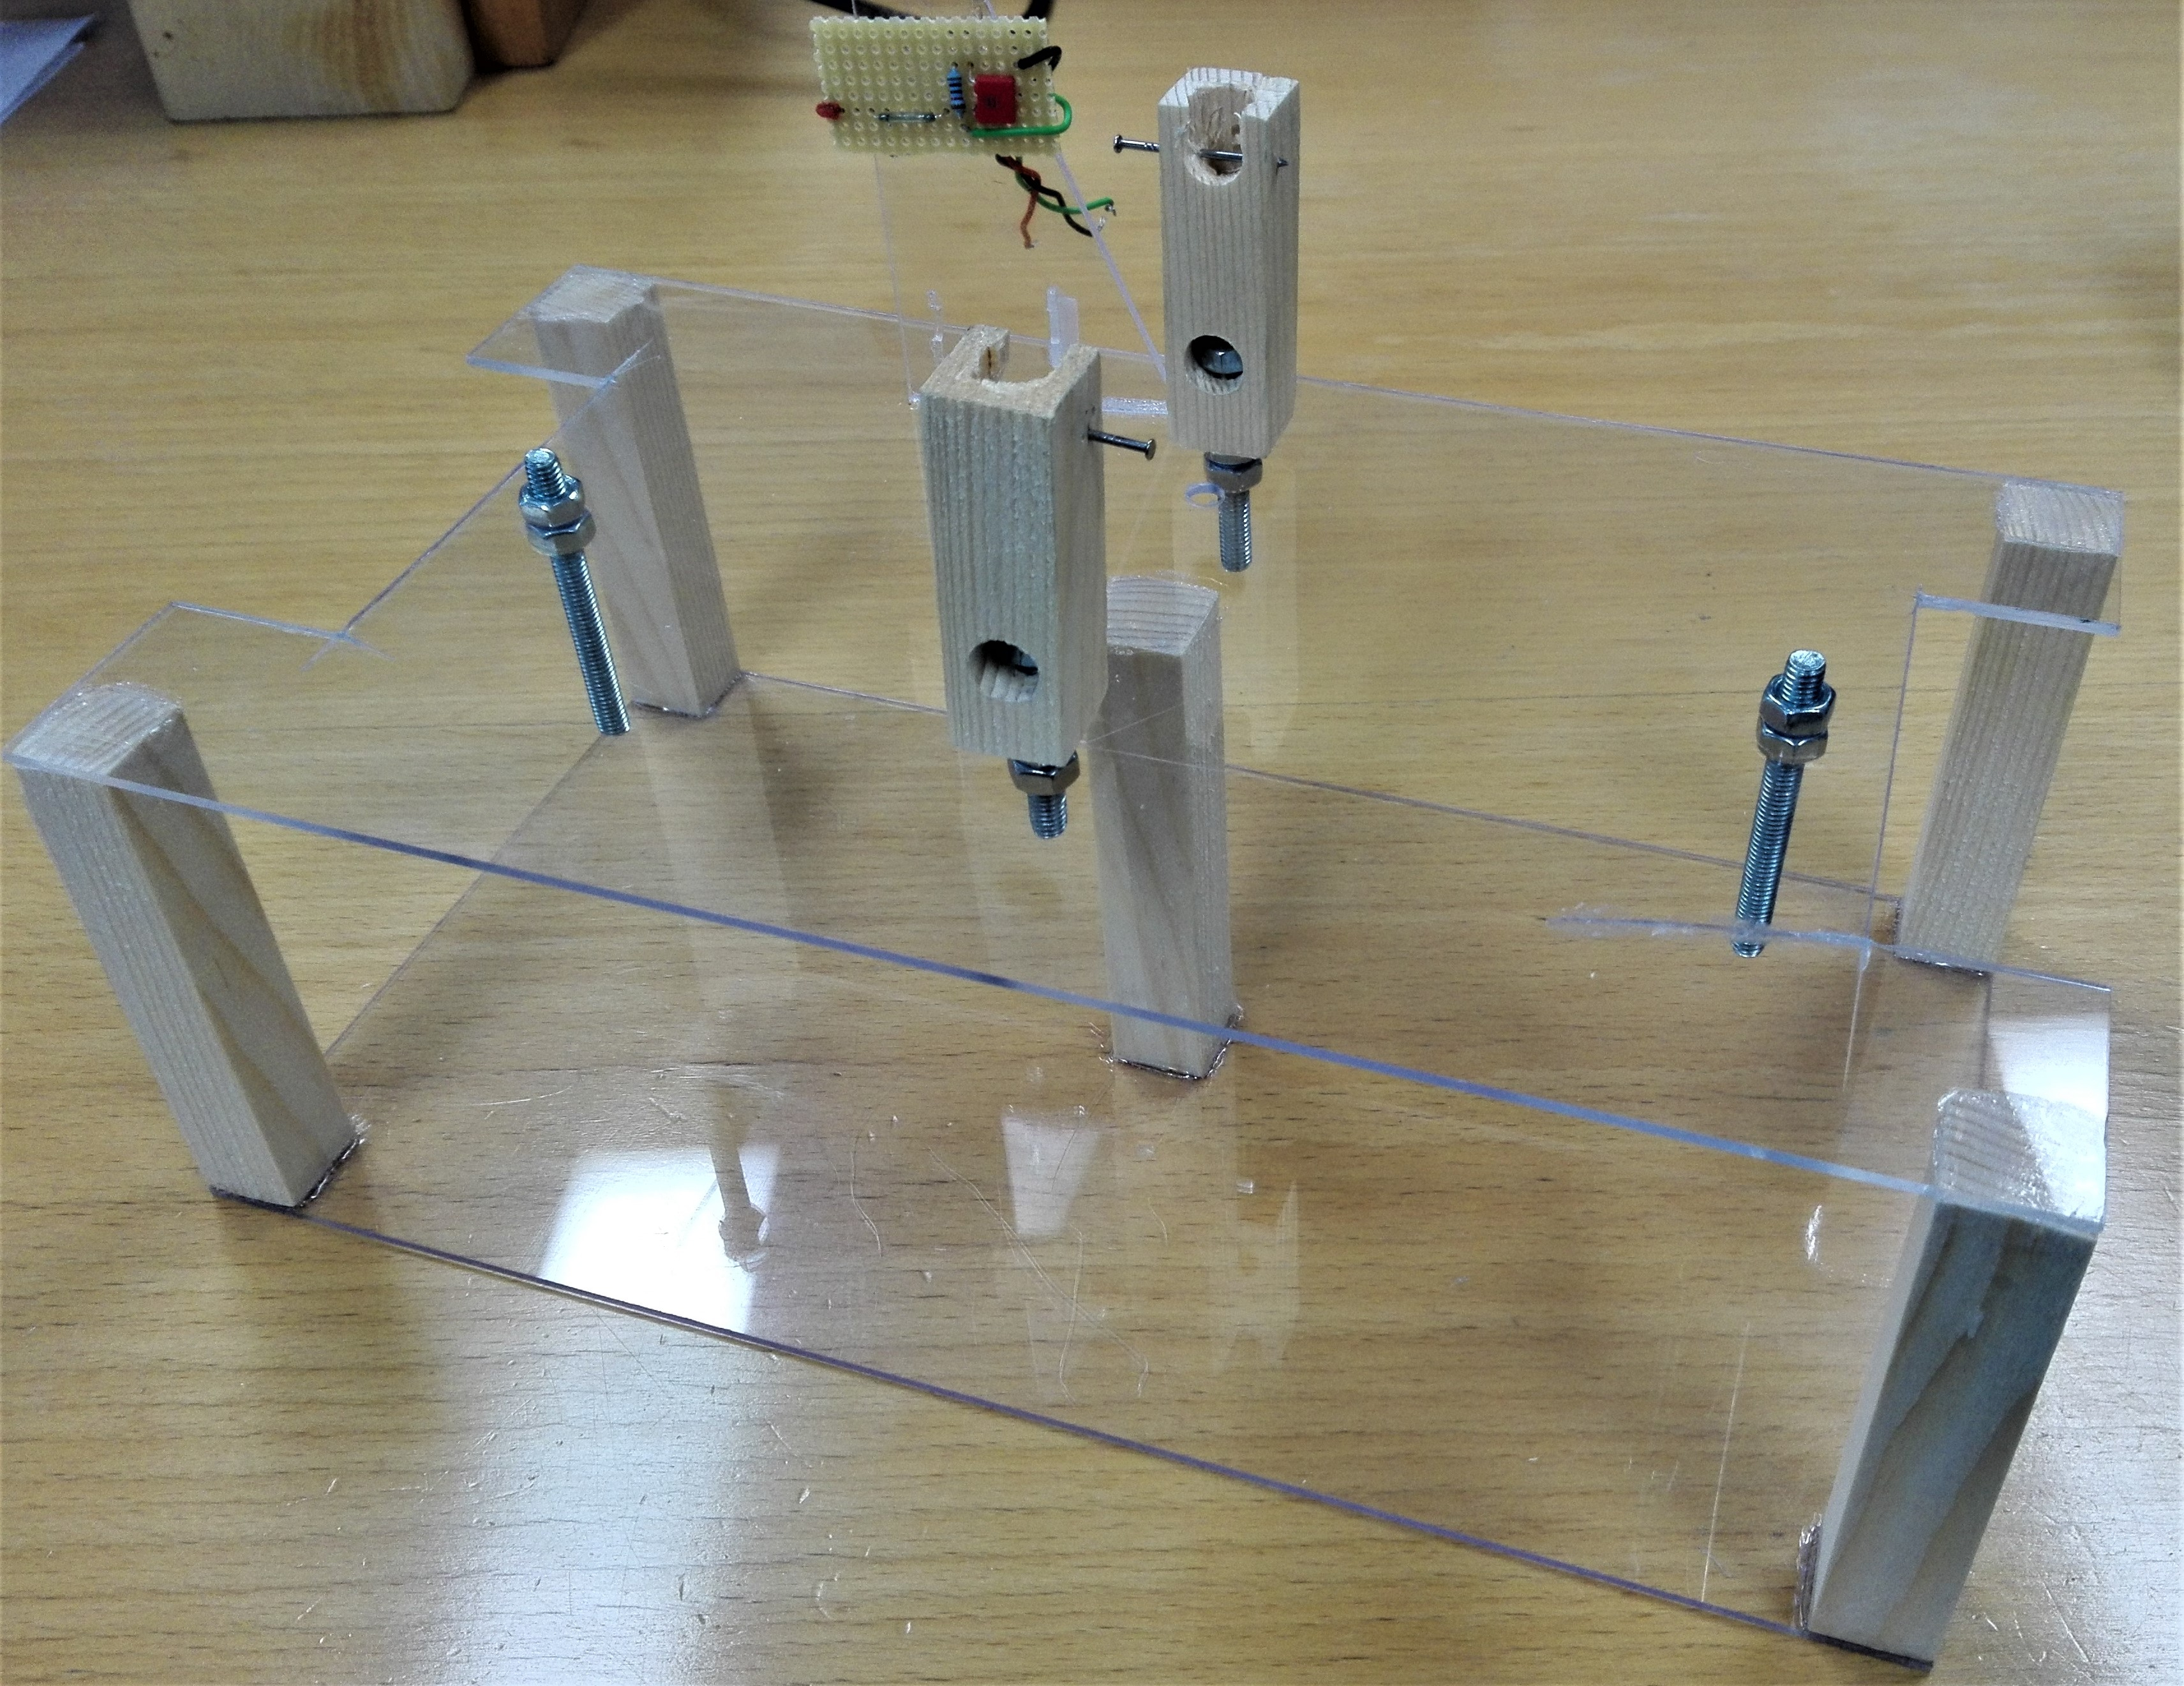
\includegraphics[width=0.8\linewidth]{graphics/Etappe2.jpg}
\caption{Selbsterstelltes Gerüst.}
\label{fig:Etappe2}
\end{figure}

Abbildung \ref{fig:Etappe2} zeigt das selbsterstellte Gerüst für die Höhenverstellbare, drehbare Lagerung des Kipplöffels. Es kann sowohl die Höhe des Kipplöffels, sowie dessen Neigung in den Endpositionen über Gewinden mit Muttern eingestellt werden. Die Schrauben des Kipplöffels kommen auf einen Stahlnagel zu liegen, womit Reibungsverluste gering gehalten werden.

\paragraph{Etappe 3: Realisierung des Trichters}
Der Trichter sorgt dafür, dass der Regen, welcher auf die Trichterfläche fällt, über der Mitte des Kipplöffels in den Löffel fliesst. Die Trichterfläche stellt gleichzeitig die Referenzfläche dar, da die gesamte Regenmenge dieser Fläche über den Kipplöffel erfasst wird. Ist diese Fläche von 1 $m^2$ abweichend, so muss in der Firmware ein Skalierungsfaktor implementiert werden, damit die Regenmenge wie gewünscht gemäss Pflichtenheft ermittelt werden kann. Der Trichter wird aus demselben Material gefertigt wie der Kipplöffel, da hier die gleichen Anforderungen gelten. Es sei angemerkt, dass der Trichter nur bei weiteren Verwendung des selbst erstellten Kipplöffels, zusammen mit dem Gehäuse der gesamten Wetterstation, erstellt wird.

\paragraph{Etappe 4: Realisierung des Gehäuses}
Das Gehäuse soll den Sensor vor ungewollten äusseren Einflüssen schützen, sowie umgebende Elektronik vor eventuellen Regenwasserspritzer. Ausserdem soll ein Schaltkreis mit Reedrelais implementiert werden, damit die Kippbewegungen von der Elektronik erfasst werden können. Es sei erwähnt, dass das Gehäuse nur bei weiteren Verwendung des selbst erstellten Sensors, zusammen mit dem Gehäuse der Wetterstation, konstruiert wird.

\paragraph{Implementierung des Schaltkreises}
Der Schaltkreis, welcher die Kippbewegungen feststellen soll, besteht im wesentlichen aus einem Reedrelais und einem Permanentmagneten. Das Reedrelais ist NO (Normally Open) und wirkt als stromkreisschliessender Schalter, sobald ein magnetisches Feld (z.B. das eines Permanentmagneten) sich in unmittelbarer Nähe befindet. Der Permanentmagnet wird auf dem Kipplöffel befestigt und das Reedrelais als Gegenstück an einem Fixpunkt in der Nähe. Wichtig dabei ist, dass das Reedrelais bei den Endpositionen des Kipplöffels nicht geschlossen ist, damit der Stromkreis geöffnet ist und Strom gespart werden kann. Das Reedrelais benötigt einen seriellen Widerstand, damit bei einem schliessen des Stromkreises kein Kurzschluss auftritt. Ausserdem soll ein Kondensator parallel zum Widerstand sein, um die Speisespannung zu glätten und so ein nutzbares Signal zu erhalten. Die Speisespannung stellt den Pegel für ein schliessen des Reedrelais, und somit auch für eine Kippbewegung dar. Um die Kippbewegungen zu zählen, kann somit entweder jede steigende oder jede fallende Flanke des Signals gezählt werden.  

\begin{figure}[h]
\centering
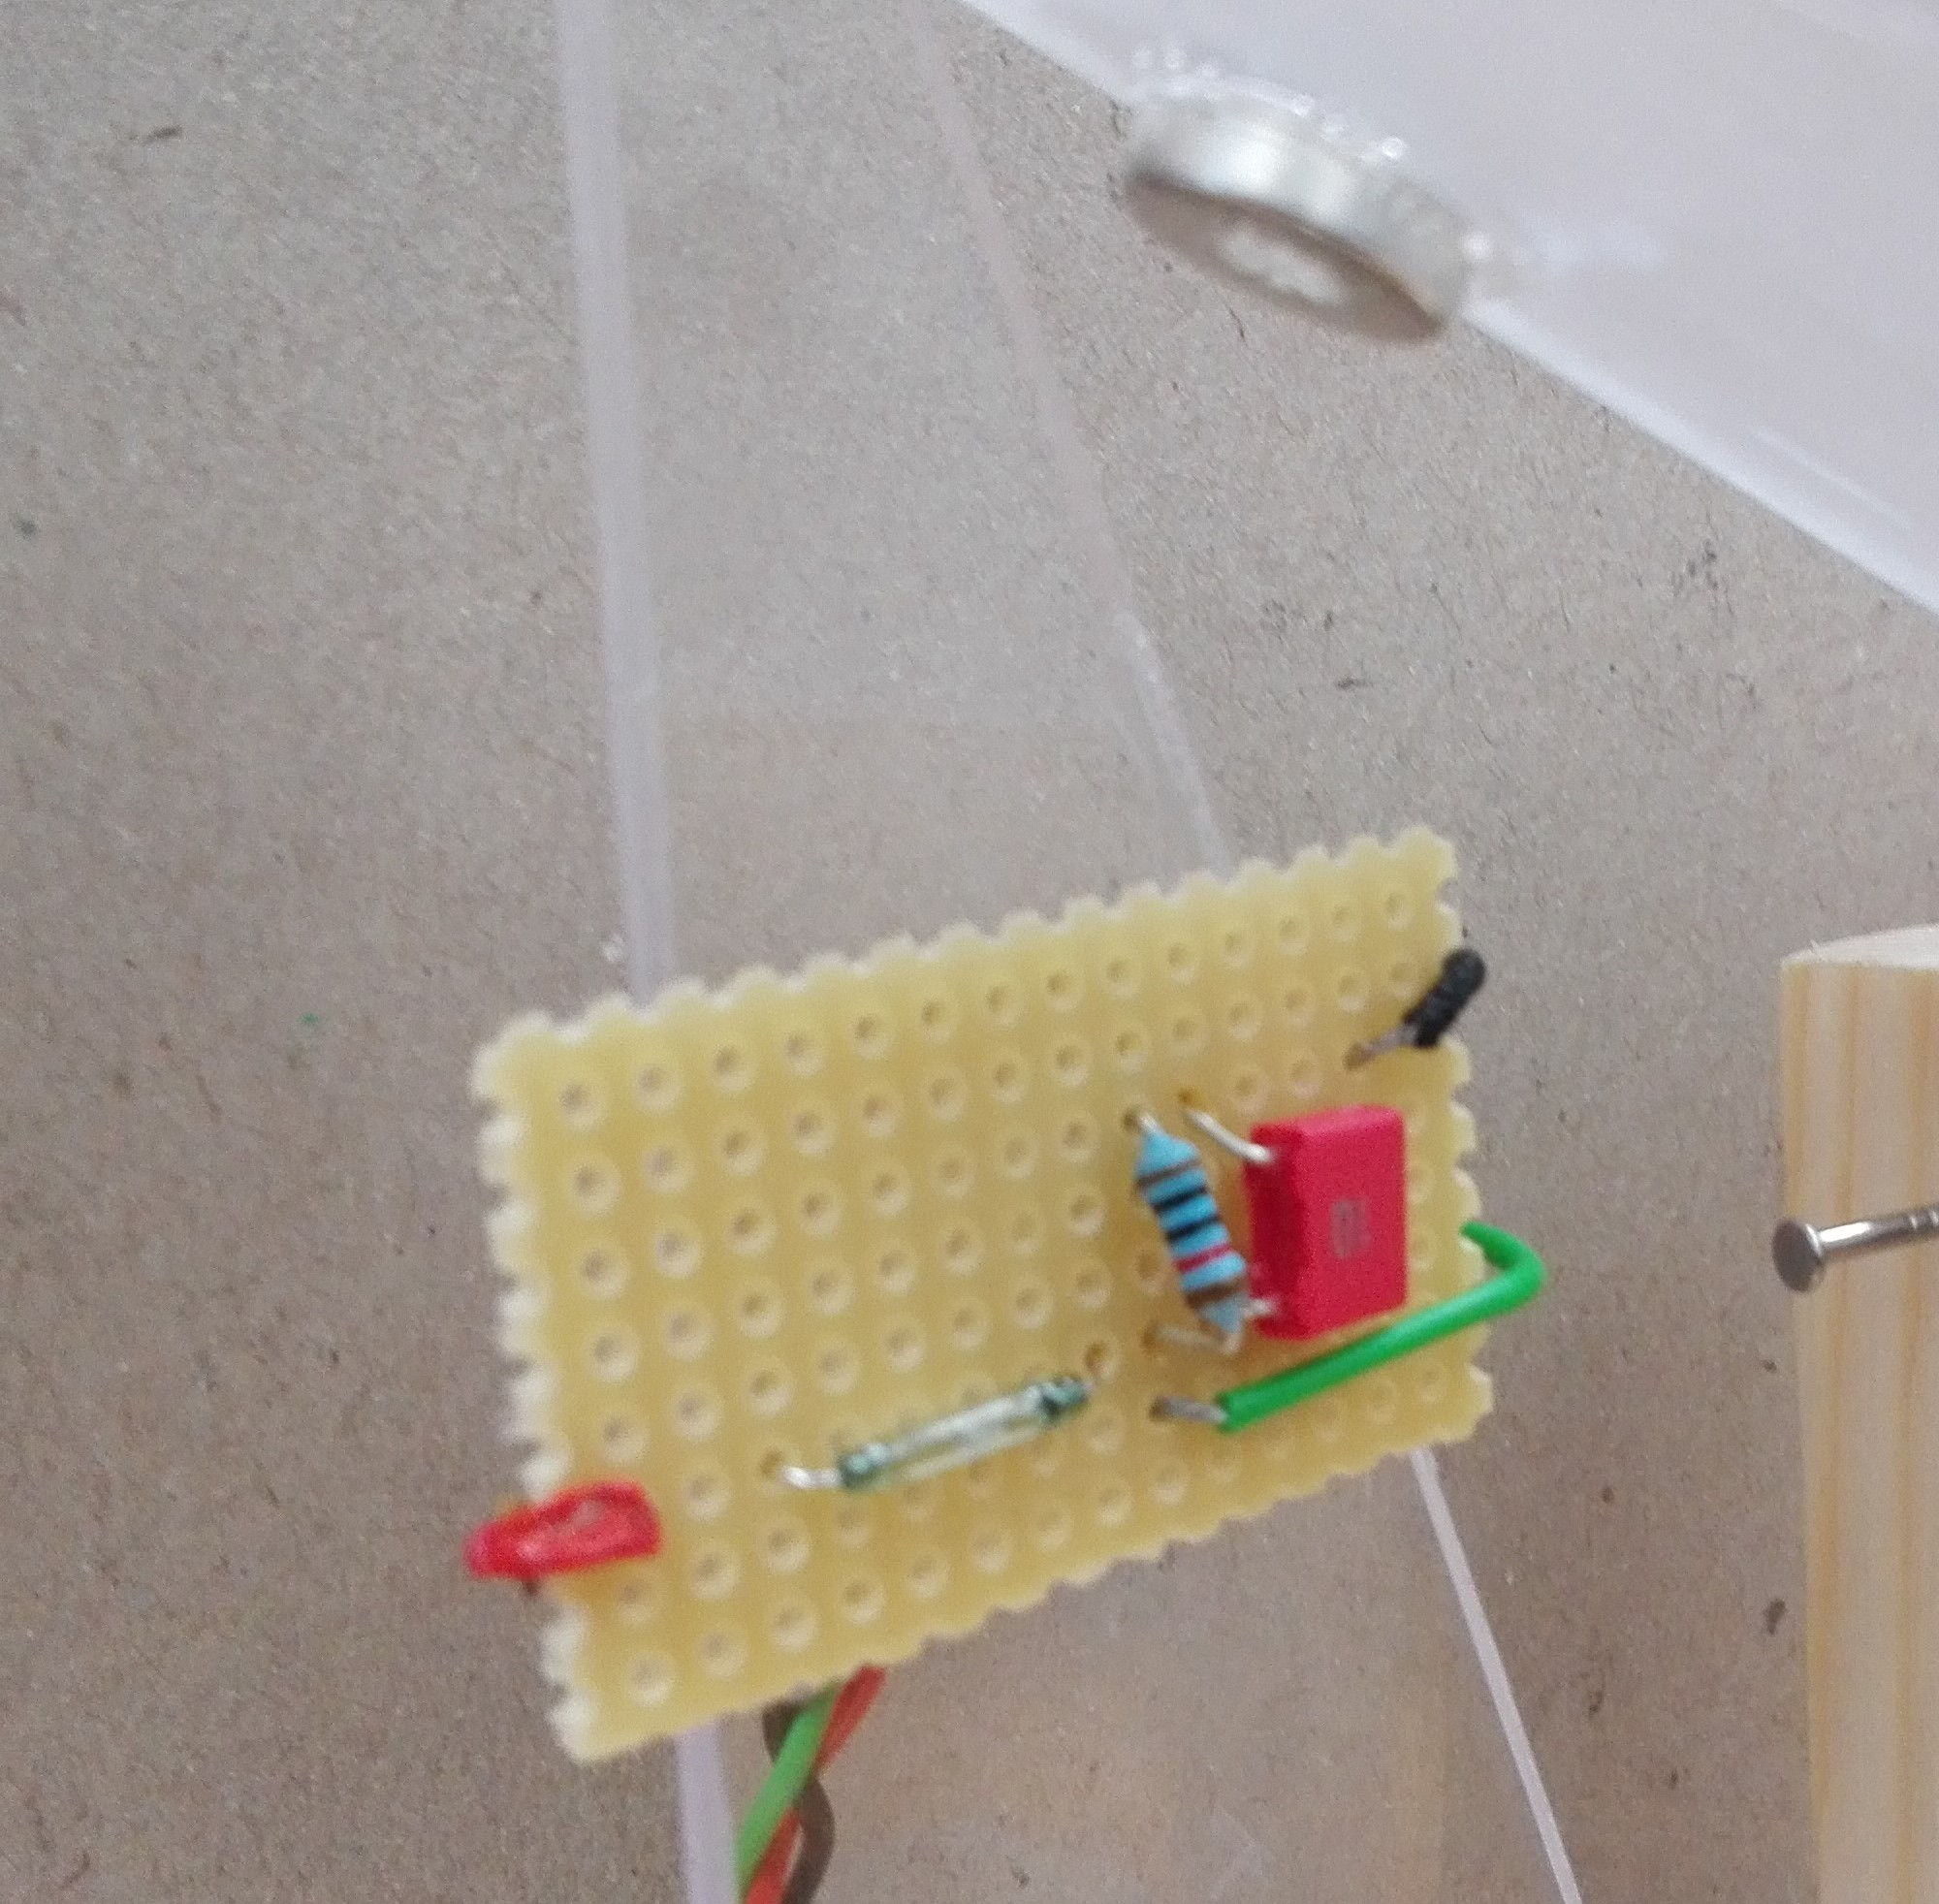
\includegraphics[width=0.4\linewidth]{graphics/KippSchalt.jpg}
\caption{Schaltkreis zur detektion der Kippbewegung.}
\label{fig:KippSchalt}
\end{figure}

Abbildung \ref{fig:KippSchalt} zeigt den Schaltkreis zur detektion der Kippbewegung. Benutzt wurde ein 10k$\Omega$ Widerstand mit einem parallel angeschlossenen 100nF Kondensator. Der Reedkontakt reagiert auf den ebenso sichtbaren Permanentmagneten, welcher an der Unterseite des Kipplöffels befestigt ist.

\newpage
\paragraph{Nachteile des Selbstgebauten Niederschlagsmengensensor}
Der selbstgebaute Niederschlagssensor beweist, dass das Prinzip des Kipplöffels funktioniert. Dennoch weist der Selbstbau Mängel auf. Der verwendete Permanentmagnet muss geklebt werden, weshalb dessen Magnetfeld massiv an stärke verliert und die Schaltung deshalb äusserst nahe angebracht werden muss. Ausserdem kam es, dadurch dass keine Werkstatt zugänglich war, zu Improvisation bei nahezu allen Fertigungsschritten, was zu unkalkulierbaren Abweichungen führt. Als Beispiel sei das Spiel der drehbaren Lagerung des Kipplöffels auf dem Gerüst angeführt, was jegliche Justierungsversuche der Niederschlagsmenge beeinflusst. Aus den genannten Gründen wird vorgefertigter Sensor mit Kipplöffelprinzip verwendet.\\

\begin{figure}[hbtp]
\centering
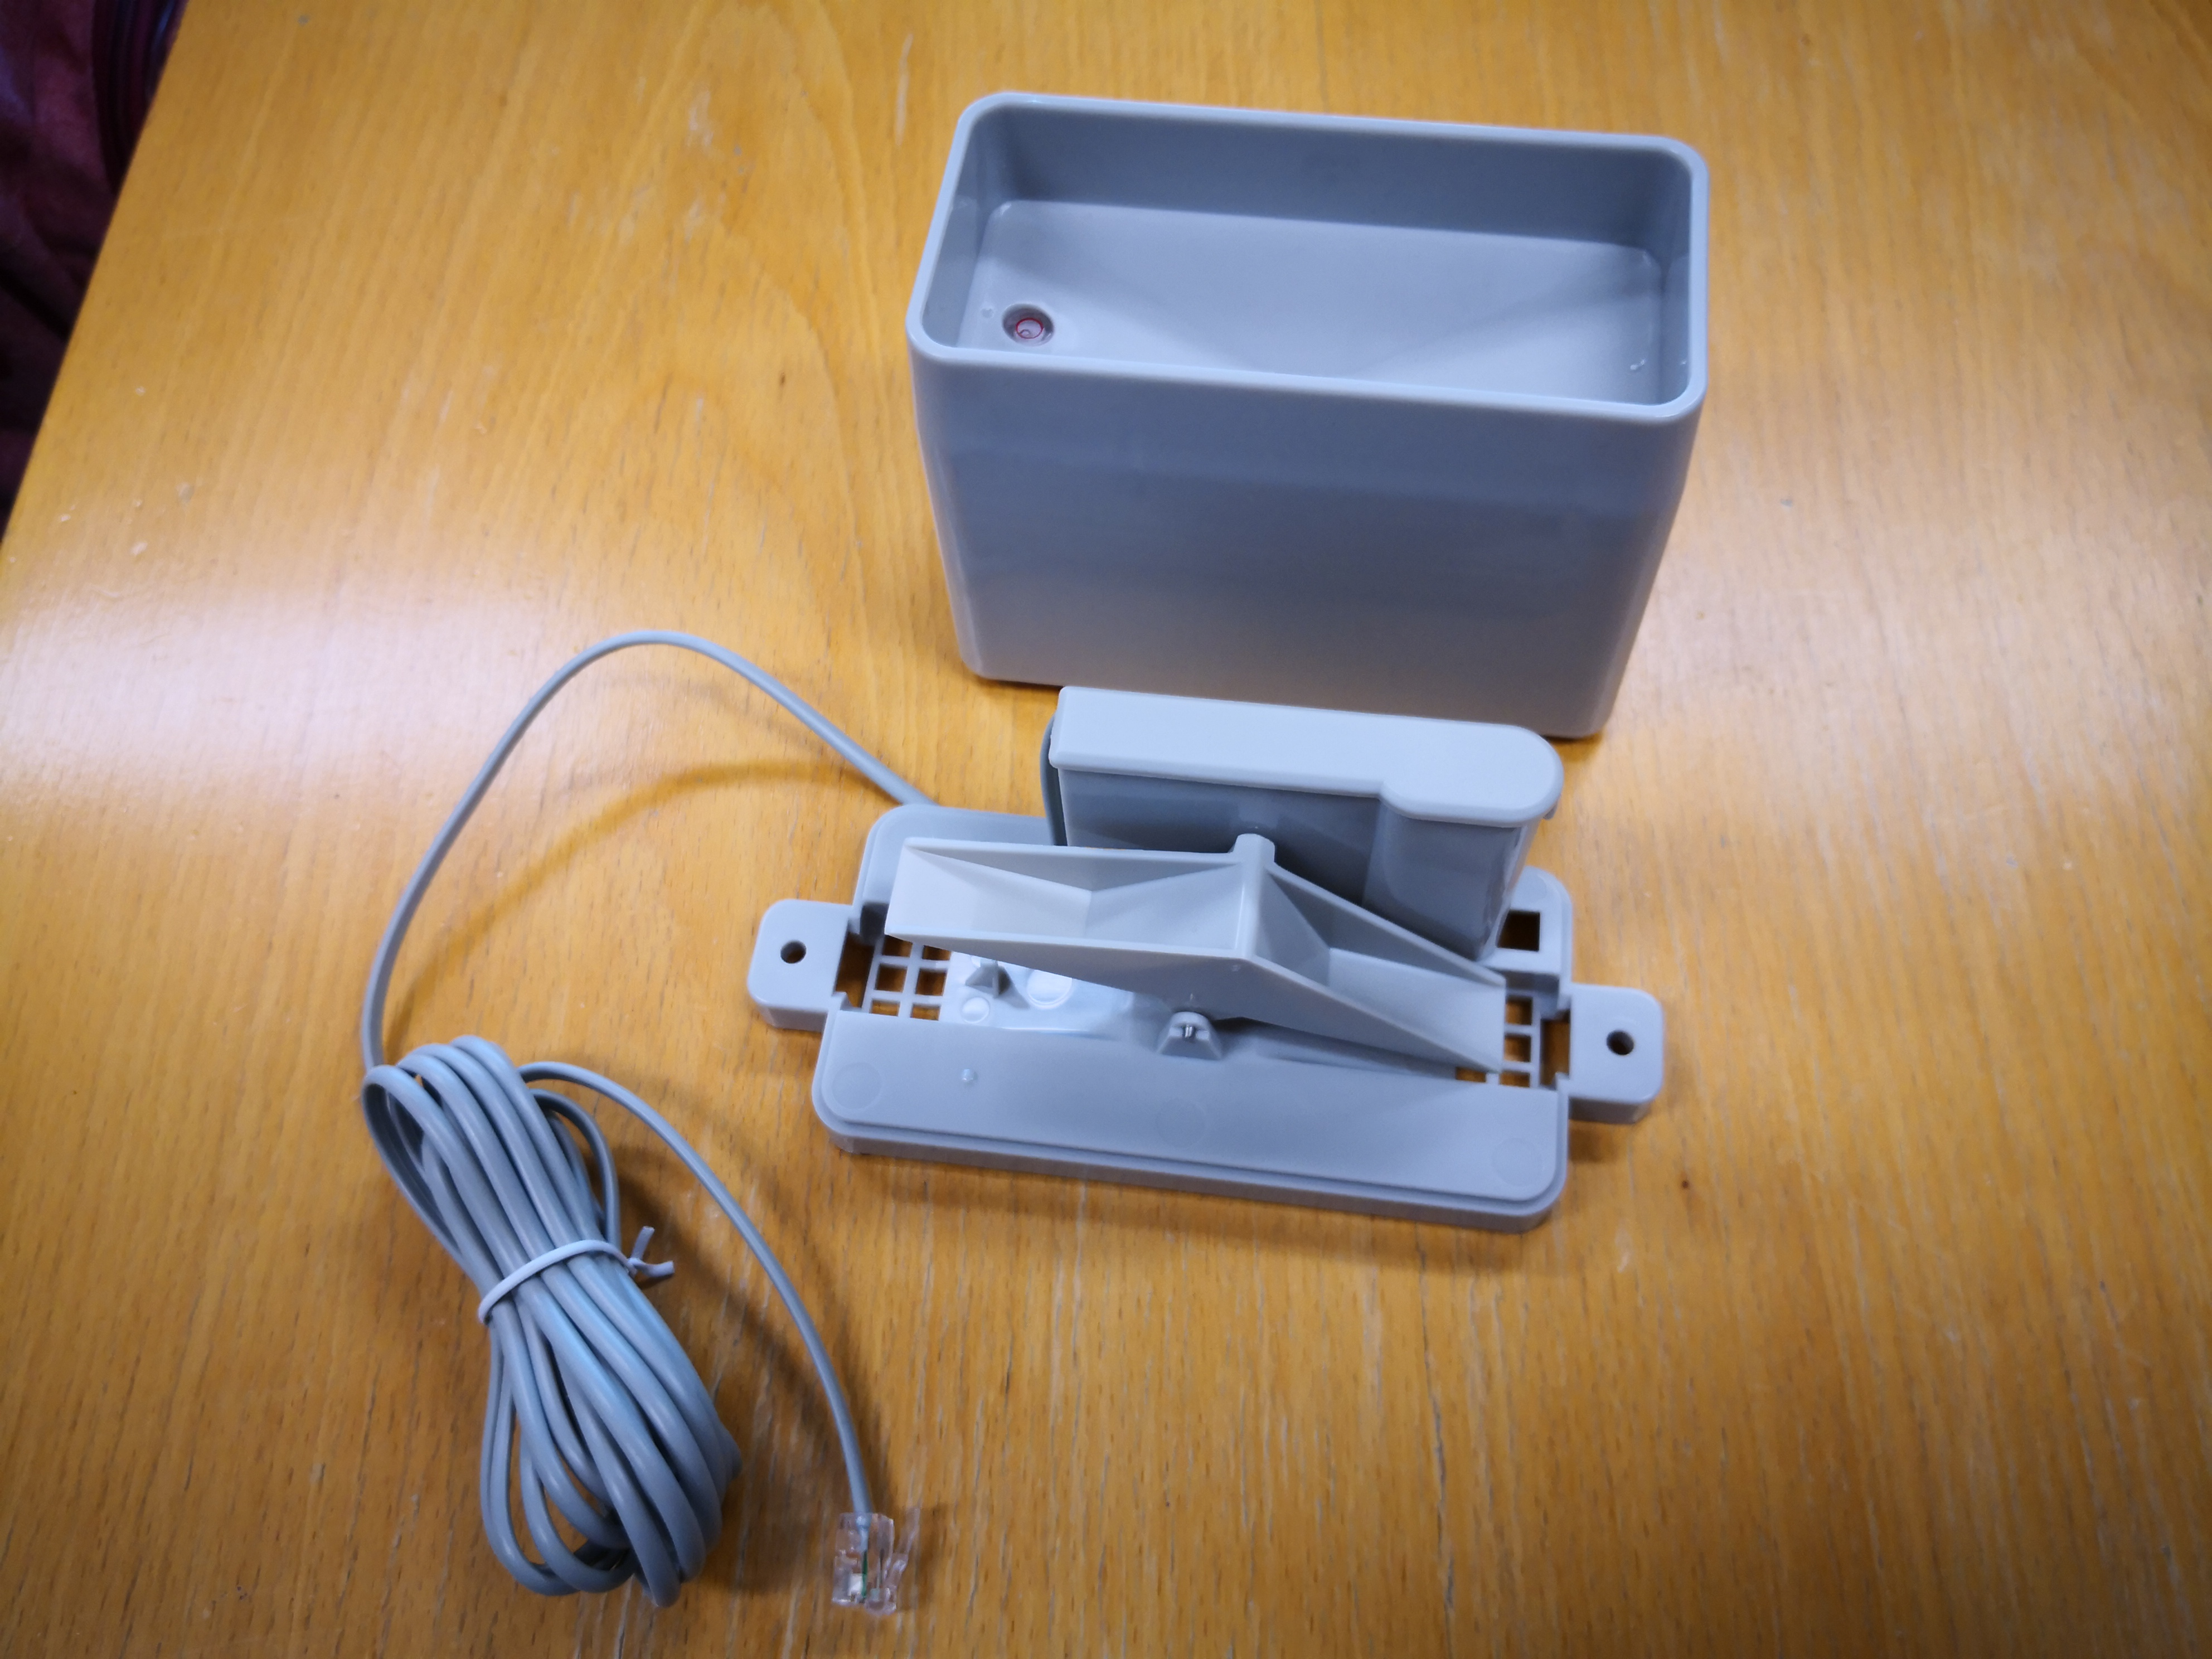
\includegraphics[width=0.7\textwidth]{graphics/ombrometer/IMG_20190118_110027.jpg}
\caption{Das Ombrometer}
\label{fig:verwendetes_ombrometer}
\end{figure}

Das verwendete Ombrometer von MISOL hat eine Auflösung von ca. 2ml pro Kippbewegung auf auf die Dimensionen $5.5E-2m*11.5E-2m$ des Trichters. Zudem enthält der Trichter oben noch eine kleine Wasserwaage, damit das Ombrometer auch gerade steht und die gemessene Regenmenge nicht verfälscht wird.\\

%\subsubsection*{Implentation in der Firmware}
%Die Implementation wurde über einen Interrupt-Pin des ATMega2560 gemacht. Jedes mal wenn der Kipplöffel des Ombrometers kippt, wird ein Interrupt der auf die steigende Flanke des anliegenden Signals getriggert ist ausgeführt, welcher einen Counter für das Ombrometer inkrementiert. Eine Kippbewegung des Ombrometers umfasst ca. 2ml auf eine Fläche von $5.5E-2m*11.5E-2m=\underline{\underline{6.325E-3m^{2}}}$. Hochgerechnet auf einen Quadratmeter ergibt sich
%\begin{equation}
%2ml*\dfrac{1m^{2}}{6.325E-3m^{2}} = \underline{\underline{316.21ml}}
%\end{equation}
%benötigter Niederschlag für eine Kippbewegung des Ombrometers pro Quadratmeter. Nun kann die Niederschlagmenge in einem bestimmten Zeitraum ausgegeben werden.\\

\subsection{Anemometer}
{\begin{minipage}[b][650pt][t]{0.55\textwidth}
Für die Windgeschwindigkeitsmessung wurde ein Ersatz Anemometer von Froggit genommen (Abb. \ref{fig:anemometer}). Das Anschlusskabel hat einen vier poligen RJ-11 Stecker, dessen Signal über eine Buchse zum MCU geführt wird. Das Anemometer selbst hat allerdings nur zwei Anschlüsse, die Speisung (rot) und das durch einen mit einem Dauermagneten schließbaren Reedkontakt modulierte pulsförmige Ausgangssignal (grün, Abb. \ref{fig:rj11stecker}). In der Abb. \ref{fig:beschaltungAnemometer} ist ersichtlich, dass das Ausgangssignal über R1 abfällt und C1 als Spannungsstabilisierung dient. Das daraus resultierende Signal ist in der Abb. \ref{fig:rechteckpuls_anemometer} aufgezeigt. Die Windgeschwindigkeit ist nun aus der Anzahl Rechteckpulsen direkt interpretierbar:\\

Wenn über einen Zeitraum $T$ die Anzahl Pulse $A$ gemessen werden, dann kann auf die Winkelgeschwindigkeit $\omega$ nach 
\begin{equation}
\centering
\omega=\frac{A}{T}\qquad[s^{-1}]
\end{equation}
geschlossen werden. Da allerdings verschiedene Faktoren wie das Trägheitsmoment des Schalenkreuzes, Reibungsverluste bei der Drehbewegung, Verfälschung bei wechselnder Windrichtung usw. zusätzlich auf das Anemometer wirken, wird es sehr komplex die Windgeschwindigkeit exakt zu berechnen. Deshalb wird nur ein Näherungswert ermittelt und mit einem Skalierungsfaktor $SF$ korrigiert. Somit ergibt sich für die Windgeschwindigkeit $v_{Wind}$ mit Radius $r$ des Schalenkreuzes
\begin{equation}
\centering
v_{Wind} = \frac{A*r*SF}{T}\qquad[m/s].
\label{equ:berechnungWindgeschwindigkeit}
\end{equation}
Der Skalierungsfaktor $SF$ wird mittels Referenzmessungen der Windgeschwindigkeit eines digitalen Anemometers eruiert. \\
\end{minipage}}
{\begin{minipage}[b][650pt][t]{0.44\textwidth}
\centering
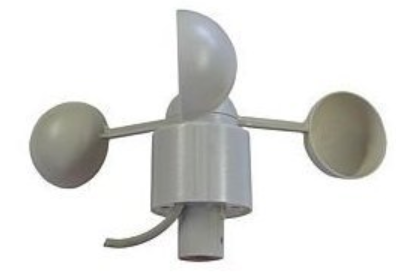
\includegraphics[width=0.9\textwidth]{graphics/Anemometer/anemometer.png}
\captionof{figure}{Anemometer \cite{AmazonAnemometer}}
\label{fig:anemometer}
\vspace{20pt}
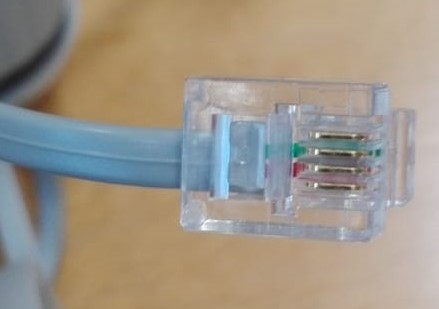
\includegraphics[width=0.9\textwidth]{graphics/Anemometer/rj_11_anschlussstecker.png}
\captionof{figure}{RJ-11 Stecker}
\label{fig:rj11stecker}
\vspace{20pt}
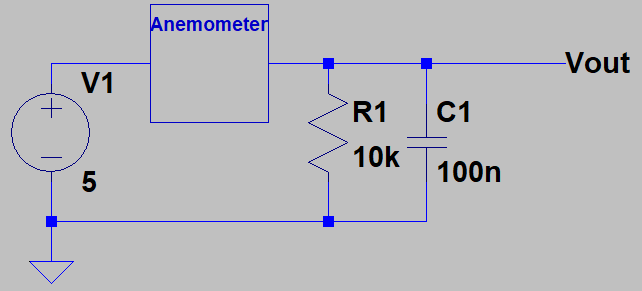
\includegraphics[width=0.9\textwidth]{graphics/Anemometer/schaltung_anemometer.png}
\captionof{figure}{Beschaltung des Ausgangs des Anemometers.}
\label{fig:beschaltungAnemometer}
\vspace{20pt}
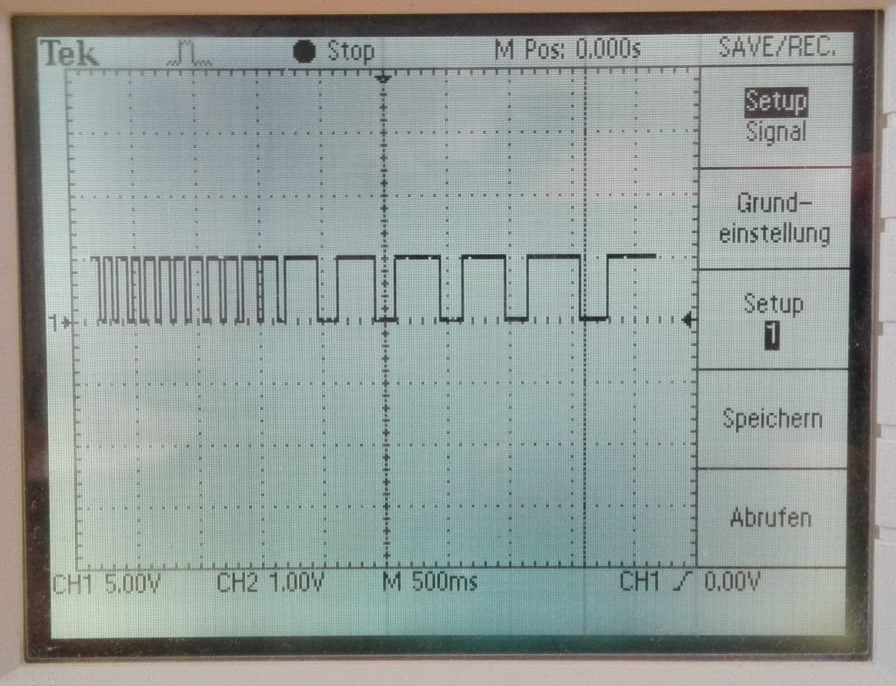
\includegraphics[width = 0.9\textwidth]{graphics/Anemometer/oszilloskop_anenometer_puls.png}
\captionof{figure}{Ausgangssignal $V_{out}$}
\label{fig:rechteckpuls_anemometer}
\end{minipage}}
\newpage

%\subsubsection*{Implementation in die Firmware}
%Die Implementation wurde recht simpel gehalten. Der gesamte implementierte Code für das Anemometer ist im Headerfile ''Anemometer.h'' extern deklariert und im File Anemometer.cpp initialisiert. Das Signal $V_{out}$ ist mit einen digital Pin des Atmega 2560 (Pinnummer 2 des Arduino Mega Boards) verbunden. Über einen Zeitraum von $5000ms$, auf die steigende Flanke getriggert, wird die Anzahl von Pulsen mittels Interrupt\footnote{es handelt sich hierbei um \textit{external Interrupts}.} gezählt. Dabei wird zuerst der Interrupt auf der Pinnummer 2 aktiviert, mit einem Delay von $5000ms$ gewartet, wobei bei jedem ausgelösten Interrupt die Funktion \textcolor{orange}{countWind}() ausgeführt und somit bei jeder steigenden Flanke um eins inkrementiert wird. Zum Schluss folgt die Deaktivierung des Interrupts und die Berechnung der Windgeschwindigkeit nach der Gleichung \ref{equ:berechnungWindgeschwindigkeit}.\\

\subsection{Windrichtungsgeber}
{\begin{minipage}[b][10cm][t]{0.55\textwidth}
Um die Windrichtung angeben zu können, wurde ein Windrichtungsgeber, wie in Abb. \ref{fig:windrichtungsgeber} gezeigt von MISOL verwendet. Er ist genau wie das Ombrometer und das Anemometer mit Reedkontakten realisiert worden (siehe Abb. \ref{fig:interne_schaltung}). Dafür sind acht Reedkontakte im Kreis angeordnet und jeder hat einen in Serie geschalteten Widerstand von unterschiedlichen Dimensionen. Der Dauermagnet kann, je nach Drehwinkel bis zu zwei Reedkontakte gleichzeitig schließen. Dies erlaubt sechzehn verschiedene Winkelpositionen und somit eine Auflösung von 22.5$^{o}$. Mit einem externen Widerstand $R=10k\Omega$ (siehe Abb. \ref{fig:aussere_beschaltung}) wird eine Spannung generiert, welche dann mit dem ADC des Microcontrollers gelesen werden kann. Der Windrichtungsgeber wird mit einer Speisespannung von $V_{+}=5V$ betrieben. Der Windrichtungsgeber hat einen vierpoligen RJ-11 Anschluss. Zudem hat er auf der unteren Seite noch eine RJ-11 Buchse, bei der das Anemometer direkt angeschlossen werden kann. Wie diese Anschlüsse gemapped sind, wird in der Abb. \ref{fig:interne_schaltung} gezeigt. \\
\end{minipage}}
{\begin{minipage}[b][10cm][t]{0.44\textwidth}
\centering
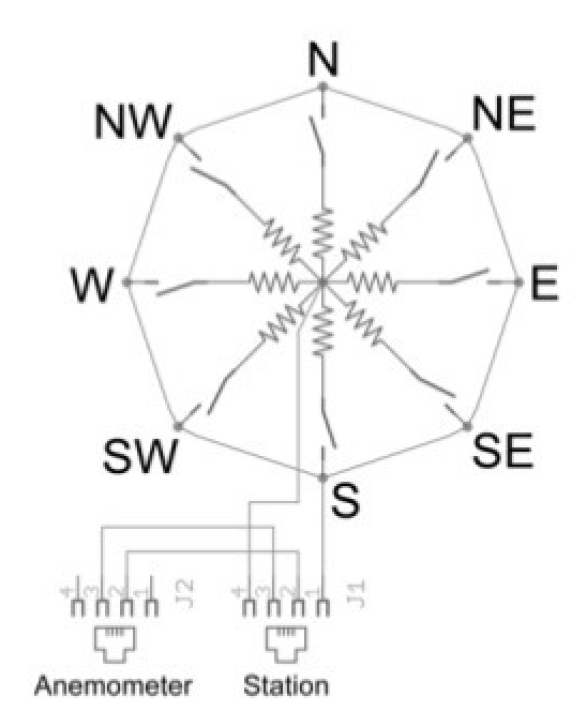
\includegraphics[width=0.9\textwidth]{graphics/windrichtungsgeber/interne_schaltung.PNG}
\captionof{figure}{Interne Schaltung \cite{ADSkeineAngabe}}
\label{fig:interne_schaltung}
\end{minipage}}

\begin{table}[h]
\centering
\caption{Technische Werte \cite{ADSkeineAngabe}}
\begin{tabular}{|c|c|c|c|}
\hline 
Richtung [$^{o}$] & Himmelsrichtung & Widerstand [$\Omega$] & Ausgangsspannung [V] \\ 
\hline 
0 & N & 33k & 3.84 \\ 
\hline 
22.5 &  & 6.57k & 1.98 \\ 
\hline 
45 & NE & 8.2k & 2.25 \\ 
\hline 
67.5 &  & 891 & 0.41 \\ 
\hline 
90 & E & 1k & 0.45 \\ 
\hline 
112.5 &  & 688 & 0.32 \\ 
\hline 
135 & SE & 2.2k & 0.90 \\ 
\hline 
157.5 &  & 1.41k & 0.62 \\ 
\hline 
180 & S & 3.9k & 1.40 \\ 
\hline 
202.5 &  & 3.14k & 1.19 \\ 
\hline 
225 & SW & 16k & 3.08 \\ 
\hline 
247.5 &  & 14.12k & 2.93 \\ 
\hline 
270 & W & 120k & 4.62 \\ 
\hline 
292.5 &  & 42.12k & 4.04 \\ 
\hline 
315 & NW & 64.9k & 4.33 \\ 
\hline 
337.5 &  & 21.88k & 3.43 \\ 
\hline 
\end{tabular} 
\label{tab:technische_werte}
\end{table}

In der Tabelle \ref{tab:technische_werte} sind die Widerstandswerte der in Abb. \ref{fig:interne_schaltung} gezeigten Widerständen und die Werte der Ausgangsspannung bei variabler Winkelposition aufgelistet. Da nun abhängig von der Winkelposition unterschiedliche Widerstände parallel geschalten werden, resultiert am Ausgang eine vom Winkel abhängige Ausgangsspannung.\\

\newpage


{\begin{minipage}[b][6cm][t]{0.49\textwidth}
\centering
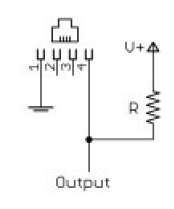
\includegraphics[width=0.5\textwidth]{graphics/windrichtungsgeber/aeussere_beschaltung.PNG} 
\captionof{figure}{Spannungsteiler mit $R=10k\Omega$ \cite{ADSkeineAngabe}}
\label{fig:aussere_beschaltung}
\end{minipage}}
{\begin{minipage}[b][6cm][t]{0.49\textwidth}
\centering
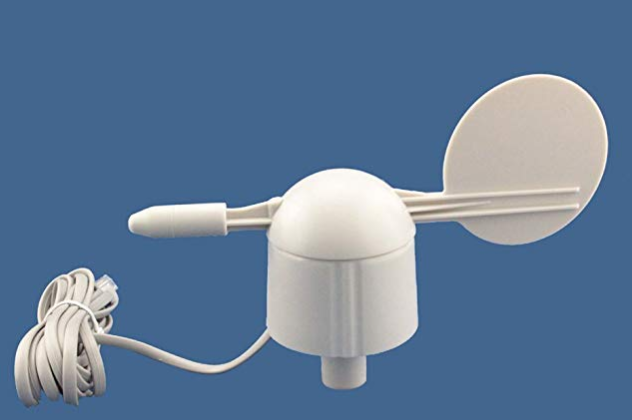
\includegraphics[width=0.9\textwidth]{graphics/windrichtungsgeber/windrichtungsgeber.PNG}
\captionof{figure}{Windrichtungsgeber von MISOL \cite{windrichtungsgeber}}
\label{fig:windrichtungsgeber}
\end{minipage}}

%\subsubsection*{Implementation in die Firmware}
%Der ADC hat des ATMega2560 hat eine 10 Bit Auflösung und wird mit 5 Volt betrieben. Um das Signal am ADC lesen zu können, wird die Funktion \textit{analogRead()} aufgerufen. Als Rückgabewert wird ein binärer Wert als Dezimalzahl vom Datentyp \textit{float} erhalten. Um diesen Wert in die eigentlich am ADC anliegende Spannung umzurechnen wird die Gleichung \ref{equ:ADC1} umgeformt.
%\begin{equation}
%\centering
%\dfrac{Auflösung ADC}{Betriebsspannung} = \dfrac{analogRead()}{Ausgangsspannung}
%\label{equ:ADC1}
%\end{equation}
%Daraus resultiert:
%\begin{equation}
%\centering
%Ausgangsspannung = \dfrac{analogRead()*Betriebsspannung}{Auflösung ADC}
%\label{equ:ADC2}
%\end{equation}
%Werden nun die Werte in die Gleichung \ref{equ:ADC2} eingefügt, ergibt sich für die Ausgangsspannung $V_{out}$:
%\begin{equation}
%\centering
%V_{out}(analogRead()) = \dfrac{analogRead()*5V}{10}
%\label{equ:adc_vout}
%\end{equation}
%Diese von \textit{analogRead()} abhängige Ausgangsspannung $V_{out}$ wird dann in \textit{if else} Anweisungen zu der Himmelsrichtung zugewiesen und als String abgespeichert.

\subsection{BME280}
\label{BME280}
{\begin{minipage}[b][6cm][t]{0.55\textwidth}
Der \textit{BME280} ist ein low powered digitaler Feuchtigkeits-, Luftdruck- und Temperatursensor von Bosch. Er ist in einem 2.5mm x 2.5mm x 0.93mm metal lid LGA Gehäuse verpackt und kann über die Interfaces I$^{2}$C und SPI kommunizieren. Durch seinen niedrigen Stromverbrauch, große operating range der drei Messgrößen und schnellen Ansprechzeit von etwa 1s eignet er sich für die solarbetriebene mobile Wetterstation besonders. \cite{Bosch2019}\\
\end{minipage}}
{\begin{minipage}[b][6cm][t]{0.44\textwidth}
\centering
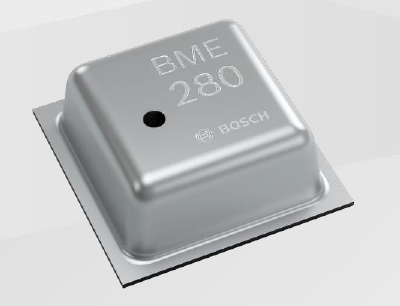
\includegraphics[width=0.9\textwidth]{graphics/bme280/bme280.PNG}
\captionof{figure}{BME280 \cite{Bosch2019}}
\label{fig:bme280}
%\vspace*{0.5cm}
%\centering
%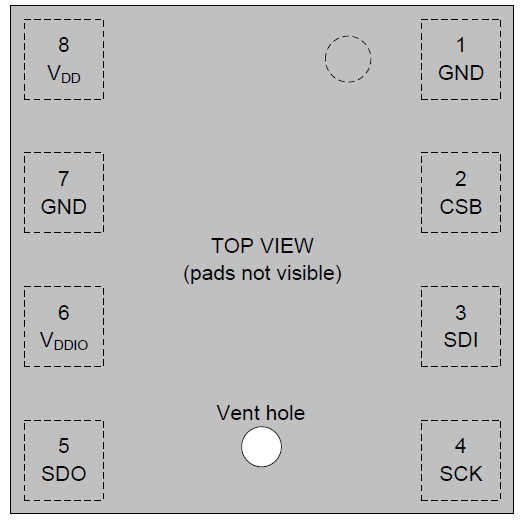
\includegraphics[width=0.9\textwidth]{graphics/bme280/bme280_pinout.PNG}
%\captionof{figure}{Pinout \cite{Bosch2019}}
%\label{fig:bme280_pinout}
\end{minipage}}

\begin{table}[h]
  \centering
  \caption{Elektrische Spezifikationen \cite{Bosch2019}}
    \begin{tabular}{lllll}
    \toprule
    \textbf{Parameter} & \textbf{Min.} & \textbf{Typ.} & \textbf{Max.} & \textbf{Einheit} \\
    \midrule
    Versorgungsspannung & 1.71  & 1.8   & 3.6   & V \\
    Stromverbrauch (sleep mode) &       & 0.1   & 0.3   & $\mu$A \\
    Stromverbrauch inaktiv (normal mode) &       & 0.2   & 0.5   & $\mu$A \\
    Stromverbrauch Feuchtigkeitsmessung &       & 340   &       & $\mu$A \\
    Stromverbrauch Luftdruckmessung &       & 714   &       & $\mu$A \\
    Stromverbrauch Temperaturmessung &       & 350   &       & $\mu$A \\
    \bottomrule
    \end{tabular}%
  \label{tab:elektrische_Spezifikationen}%
\end{table}%

Bei einer Messfrequenz von 1Hz für die drei Messgrößen verbraucht der BME280 somit laut Datenblatt nur \textbf{3.6$\mu$A}. \cite[S. 2]{Bosch2019}

\subsubsection*{Feuchtigkeitsmessung}
In der Tabelle \ref{tab:spez_feuchtigkeit} sind die wichtigsten Parameter zur Feuchtigkeitsmessung aufgelistet. Zu vermerken ist, dass die digitalen Werte des BME280 zur Feuchtigkeitsmessung relativ sind und deshalb prozentual angegeben werden. \\
\begin{table}[htbp]
  \centering
  \caption{Sezifikationen der Feuchtigkeitsmessung \cite{Bosch2019}}
    \begin{tabular}{lllll}
    \toprule
     \textbf{Parameter} & \textbf{Min.} & \textbf{Typ.} & \textbf{Max.} & \textbf{Einheit} \\
    \midrule
    Operating range & -40   & 25    & 85    & $^{o}$C \\
          & 0     &       & 100   & \% \\
    Absolute Genauigkeitstoleranz &       & $\pm$3 &       & \% \\
    Hysterese &       & $\pm$1 &       & \% \\
    Auflösung &       & 0.008 &       & \% \\
    Langzeitstabilität &       & 0.5   &       & \% pro Jahr \\
    \bottomrule
    \end{tabular}%
  \label{tab:spez_feuchtigkeit}%
\end{table}%

\newpage

\subsubsection*{Luftdruckmessung}
Die Genauigkeit der Luftdruckmessung ist an einen Temperaturbereich gebunden. Bei niedrigeren Temperaturen (<0$^{o}$C) weist der Sensor eine höhere Unsicherheit auf als bei Temperaturen von 0 bis 65 $^{o}$C (siehe Tabelle \ref{tab:spez_druck}). \\
\begin{table}[htbp]
  \centering
  \caption{Sezifikationen der Luftdruckmessung \cite{Bosch2019}}
    \begin{tabular}{llllll}
    \toprule
    \textbf{Parameter} & \multicolumn{1}{l}{\textbf{Temperaturbereich}} & \multicolumn{1}{l}{\textbf{Min.}} & \textbf{Typ. } & \multicolumn{1}{l}{\textbf{Max.}} & \textbf{Einheit} \\
    \midrule
    Operating range &       & \multicolumn{1}{l}{-40} & 25    & \multicolumn{1}{l}{85} & $^{o}$C \\
          &       & 300   &       & 1100  & hPa \\
    Absolute Genauigkeit & \multicolumn{1}{c}{-20 bis 0 $^{o}$C} &       & $\pm$1.7 &       & hPa \\
          & \multicolumn{1}{c}{0 bis 65 $^{o}$C} &       & $\pm$1  &       & hPa \\
    Auflösung &       &       & \multicolumn{1}{r}{0.18} &       & hPa \\
    Langzeitstabilität &       &       & $\pm$1  &       & hPa pro Jahr \\
    \bottomrule
    \end{tabular}%
  \label{tab:spez_druck}%
\end{table}%

\subsubsection*{Temperaturmessung}
Die Wetterstation wird hauptsächlich in einem Temperaturbereich von 0 bis 65 $^{o}$C betrieben, wodurch vom Sensor eine Unsicherheit von max. $\pm$1 $^{o}$C erreicht werden kann. \\
\begin{table}[htbp]
  \centering
  \caption{Sezifikationen der Temperaturmessung \cite{Bosch2019}}
    \begin{tabular}{llllll}
    \toprule
    \textbf{Parameter} & \multicolumn{1}{l}{\textbf{Temperaturbereich}} & \multicolumn{1}{l}{\textbf{Min.}} & \textbf{Typ. } & \multicolumn{1}{l}{\textbf{Max.}} & \textbf{Einheit} \\
    \midrule
    Operating range &       & \multicolumn{1}{l}{-40} & 25    & \multicolumn{1}{l}{85} & $^{o}$C \\
    Absolute Genauigkeit & \multicolumn{1}{c}{25 C} &       & $\pm$0.5 &       & $^{o}$C \\
          & \multicolumn{1}{c}{0 bis 65 C} &       & $\pm$1  &       & $^{o}$C \\
          & \multicolumn{1}{c}{-20 bis 0 C} &       & $\pm$1.25 &       & $^{o}$C \\
          & \multicolumn{1}{c}{-40 bis -20 C} &       & $\pm$1.5 &       & $^{o}$C \\
    Auflösung  &       &       & 0.01  &       & $^{o}$C \\
    \bottomrule
    \end{tabular}%
  \label{tab:spez_temp}%
\end{table}%

%\subsubsection*{Implementation in die Firmware}
%Um den BME280 vom Microcontroller aus ansteuern zu können, wurden zwei bereits existierende Librarys von Adafruit verwendet:
%\begin{itemize}
%\item Adafruit BME280 Library
%\item Adafruit Unified Sensors
%\end{itemize}
%Anschließend konnten die Headerfiles <Adafruit\_Sensor.h> und <Adafruit\_BME280.h> inkludiert werden und der Sensor über das I$^{2}$C Interface mit den folgenden Funktionen abgefragt werden:\\
%\begin{itemize}
%\item \textcolor{blue}{float} \textcolor{orange}{readTemperature}()
%\item \textcolor{blue}{float} \textcolor{orange}{readHumidity}()
%\item \textcolor{blue}{float} \textcolor{orange}{readPressure}()
%\end{itemize}

\section{Ergänzungen aus der Bachelor-Thesis}
Während der Bachelor-Thesis soll ein Sensor zur Ermittlung der Sonnenstunden implementiert werden. Um dies zu erreichen wurde die Idee, die Sonnenstunden direkt über den Ladestrom der Photovoltaikanlage zu eruieren, verworfen, da auf diese Weise mit höheren Energieverlusten zu rechnen wäre durch das Abzweigen des Ladestroms und die damit verbundene zusätzliche Speisung der Schaltung. Stattdessen wird über ein Lichtintensitätssensor die Bestrahlungsstärke gemessen, womit die Sonnenstunden über einen Schwellwert berechnet werden können. Im folgenden Abschnitt wird der verwendete Lichtintensitätssensor näher erläutert.

\subsection{Lichtintensitätssensor}
Die Lichtintensität wird über den TSL2561, ein digitaler low power Sensor, eruiert. Dieser misst über eine Kombination aus einer Breitband-Photodiode und einer Infrarot-Photodiode die Lichtstärke mit einer 16-Bit Auflösung. Über zwei integrierte AD-Wandler wird der Photodiodenstrom gewandelt und auf einen digitalen Ausgang gegeben. Über eine I$^{2}$C Schnittstelle kann dieser Ausgang auf die MCU gegeben und so ausgewertet werden. Ab einem bestimmten Schwellenwert kann die Einstrahlung als direkte Sonnenstrahlung definiert, und so auch gezählt werden. Der erwähnte Schwellenwert ist vom Ort abhängig an dem die Wetterstation sich befindet und muss eruiert und in der Firmware eingestellt werden, was im entsprechenden Teil (\refname{part:Firmware} \ref{part:Firmware})) erläutert wird. Da dieser Sensor nicht direkt auf der Platine sondern am oberen Teil des Gehäuses montiert werden muss, wird der TSL2561 als Breakout Board (Abbildung \ref{fig:TSL}) verwendet und über Pinheader mit dem PCB verbunden. Die wichtigsten elektrischen Spezifikationen sind in der Tabelle \ref{tab:TSL2561} zusammengefasst. \cite{TSL2561}\\

\begin{figure}[hbtp]
\centering
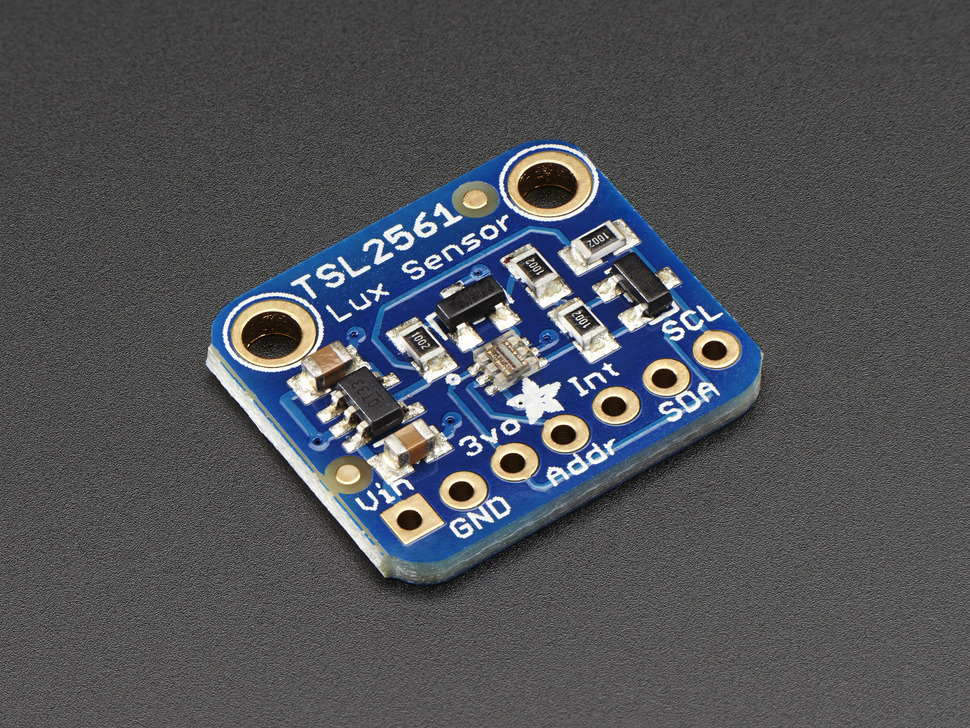
\includegraphics[width=0.5\textwidth]{graphics/TSL2561/TSL2561_Breakout.JPG}
\captionof{figure}{TSL2561 Breakout Board von Adafruit \cite{TSL2561Adafruit}}
\label{fig:TSL}
\end{figure}

\begin{table}[h]
  \centering
  \caption{Elektrische Spezifikationen des TSL2561 \cite{TSL2561}}
    \begin{tabular}{lllll}
    \toprule
    \textbf{Parameter} & \textbf{Min.} & \textbf{Typ.} & \textbf{Max.} & \textbf{Einheit} \\
    \midrule
    Versorgungsspannung & 2.7  & 3   & 3.6   & V \\
    Stromverbrauch (Aktiv) &       & 0.24   & 0.6   & mA \\
    Stromverbrauch inaktiv (Power down) &       & 3.2   & 15 & $\mu$A \\
    \bottomrule
    \end{tabular}%
  \label{tab:TSL2561}%
\end{table}%

\subsection{BME280}
Im Verlauf der Bachelor-Thesis wurde über das Design des Gehäuses der Wetterstation diskutiert, dabei wurde ebenfalls die Notwendigkeit eines Zugangs zu frischer Umgebungsluft für den BME280 erwähnt. Würde der BME280 auf dem PCB angebracht werden, so würde dieser durch die Abwärme der Elektronik stärker beeinflusst und Fehlmessungen generieren. Aus diesem Grund soll der BME280 an der unteren Seite des Gehäuses, zugänglich zu frischer Aussenluft, montiert werden. Damit Fehlmessungen möglichst vermieden werden können, wird wie beim TSL2561 für den BME280 ein Breakout Board verwendet (Abbildung \ref{fig:BME_Breakout}) und über Pinheader mit dem PCB verbunden.\\

\begin{figure}[hbtp]
\centering
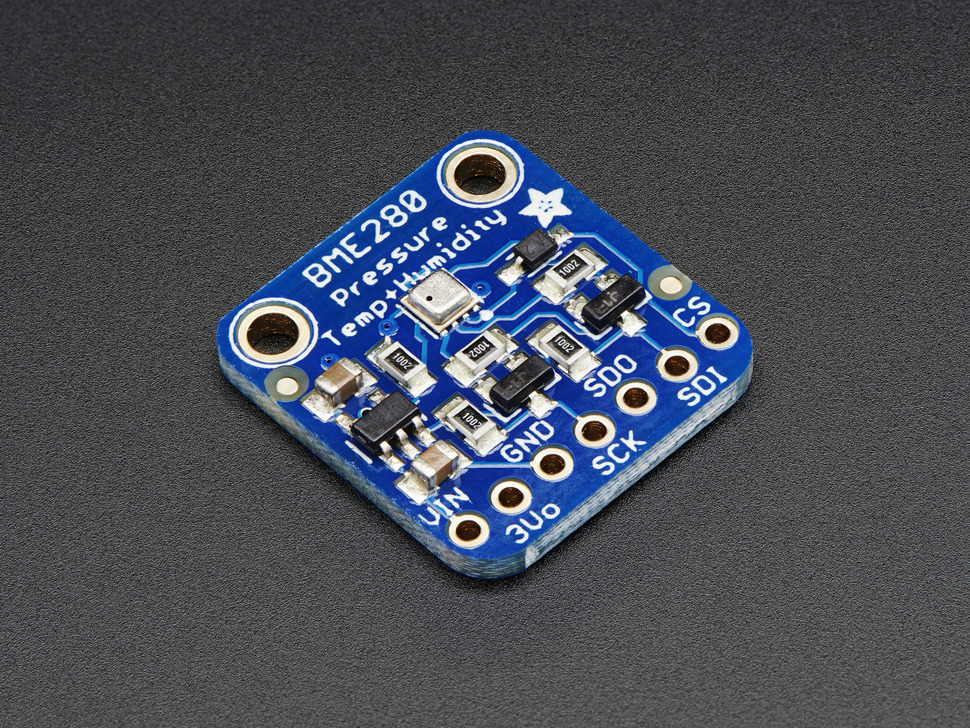
\includegraphics[width=0.5\textwidth]{graphics/BME280/BME280_Breakout.JPG}
\captionof{figure}{BME280 Breakout Board von Adafruit \cite{BME_Breakout}}
\label{fig:BME_Breakout}
\end{figure}
\subsection{Datenspeicherung}
\label{subsec:Datenspeicherung}
Während des Projekt 5 wurde die Datenspeicherung bereits mittels Breakout Board im Prototyp implementiert. Nachfolgend wird die Dokumentation aus dem Fachbericht des Projekt 5 übernommen und in einem weiteren Abschnitt Ergänzungen dazu aus der Bachelor-Thesis erläutert.

\subsubsection{Datenspeicherung - Projekt 5}
Die Datenspeicherung beinhaltet die gespeicherten Messwerte der Sensoren. Die Daten werden dann in einem *.txt-File nicht flüchtig gespeichert. Bei Beschädigung der Hardware können dann die zuletzt erfassten Daten immer noch mittels eines SD-Karten-Adapters von einem Computer ausgelesen werden. Als Kommunikationsprotokoll für das Schreiben und Auslesen der Karte wird SPI verwendet.

\subsubsection*{$\mu$SD-Karte}
\begin{minipage}{0.44\textwidth}
\centering
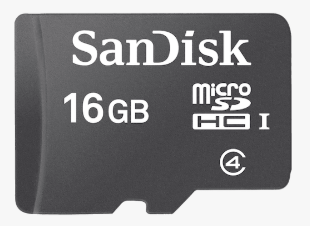
\includegraphics[width=0.4\textwidth]{graphics/Datenspeicherung/micro_sd_card_16GB.png}
\captionof{figure}{16 GB $\mu$SD-Karte \cite{musdkarte}}
\label{fig:muSDKarte}
\end{minipage}
\begin{minipage}{0.55\textwidth}
Bei der $\mu$SD-Karte muss auf die Kompatibilität mit dem Breakoutboard geachtet werden. Dafür sind folgende Kriterien zu beachten:\\
\begin{itemize}
\item Die $\mu$SD-Karte muss FAT16 oder FAT 32 formatiert sein.
\item Es sind nur die SD und SD High Capacity (SDHC) kompatibel.\\
\end{itemize}
\end{minipage}
Für die Umsetzung dieses Projektes wurde eine $\mu$SD-Karte der SD-Familie SDHC \Romannum{1} verwendet (siehe Abb. \ref{fig:muSDKarte}). SDHC sind Kapazitäten bis zu 32GB möglich und FAT32 formatiert. \cite{muSDspez}\\ 
Die Grösse eines Strings lässt sich nach der Gleichung \ref{equ:berechnung_stringgroesse} berechnen, wenn angenommen wird, dass jeder Buchstaben (char) 8 Bit hat und zum Schluss noch ein Terminator für das Stringende angehängt wird:
\begin{equation}
\centering
Anzahl\ Zeichen * 1\ Byte + 1 = String\ Grösse\ in\ Byte
\label{equ:berechnung_stringgroesse}
\end{equation}
Bei einer Speicherung der Daten nach der Struktur in Abb. \ref{fig:datenausgabe} würden somit leicht aufgerundet ca. 216 Byte pro Speichersatz benötigt werden.\\
\todo{Kontrolle ref fig:datenausgabe}
Da momentan eine 16GB grosse $\mu$SD-Karte verwendet wird, ergeben sich daraus
\begin{equation}
\dfrac{16E9}{216}=74.1E6 \approx \underline{\underline{74E6}}
\end{equation}
Speichersätze. Würden in einem zehn Minuten Zeitintervall ein Speichersatz abgespeichert werden, dann könnten 1411 Jahre 40 Wochen 4 Tage 21 Stunden 20 Minuten lang Werte von der Wetterstation abgespeichert werden. Diese Anzahl könnte noch verdoppelt werden, da wie oben bereits erwähnt $\mu$SD-Karten bis zu 32GB kompatibel sind.\\
\newpage
\subsubsection{Ergänzungen aus der Bachelor-Thesis}
Im Gegensatz zum Prototyping wird für die endgültige Wetterstation kein Breakout Board mehr verwendet. Die $\mu$SD-Karte wird in ein $\mu$SD-Karten-Adapter (Speicherkartenverbinder) gesteckt, welcher über ein Buffer (74HC4050) mit der MCU verbunden ist (siehe Abbildung \ref{fig:Uebersicht_PCB_MCU_RTC_SD_Sense}). Der 74HC4050 kann als Levelshifter verwendet werden und als Treiber für kapazitive Ladungen. In unserem Fall werden MCU und Speicherkartenverbinder mit 3.3V betrieben, weshalb kein Levelshifter notwendig ist. Der 74HC4050 wird demnach bei der Wetterstation als Treiber für kapazitive Ladungen verwendet.\\

Die Daten werden mit der Sensorik ermittelt, über die MCU verarbeitet und in der $\mu$SD-Karte gespeichert. Nun sollen die Daten jedoch per SMS (GSM) abrufbar sein und die Wetterstation ebenfalls über ein GPS-Modul verfügen. Aus diesem Grund wird im nächsten Kapitel auf die Kommunikationsmodule (GSM, GPS) eingegangen.
 
\subsection{Kommunikationsmodule}
\label{subsec:Kommunikationsmodule}
Gemäss Auftraggeber sollen Daten der Wetterstation per SMS abrufbar und der Standort der Wetterstation ermittelbar sein. Um SMS empfangen und auch senden zu können, wird ein GSM-Modul benötigt. Weiter wird ein GPS-Modul benötigt, um eine Standortermittlung durchführen zu können. Der SIM808 ist ein Kombinationsmodul aus GSM und GPS, was nicht nur Platz auf dem PCB, sondern auch Energietechnisch und Preislich Vorteile bietet, da nur ein Modul betrieben werden muss. Aus diesen Gründen wurde der SIM808 implementiert.

\subsubsection{SIM808}
{\begin{minipage}[b][6cm][t]{0.52\textwidth}
Der SIM808 (Abbildung \ref{fig:SIM808}) verfügt über GSM/GPRS (Global System for Mobile Communications / General Packet Radio Service), GPS (Global Positioning System) und BT (Bluetooth). Für die Wetterstation wird das GSM und das GPS verwendet. Tabelle \ref{tab:SIM808} zeigt die elektrischen Spezifikationen des SIM808. \cite{SIM808}\\
\end{minipage}}
{\begin{minipage}[b][6cm][t]{0.47\textwidth}
\centering
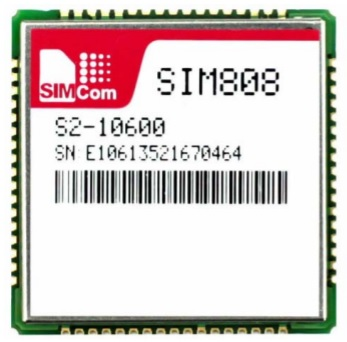
\includegraphics[width=0.7\textwidth]{graphics/SIM808/SIM808.JPG}
\captionof{figure}{SIM808 von Vorne 
\cite{SIM808}}
\label{fig:SIM808}
\end{minipage}}


\begin{table}[h]
\centering
  \caption{Elektrische Spezifikationen des SIM808 \cite{SIM808}}
\begin{tabular}{lllll}
\toprule 
\textbf{Parameter} & \textbf{Min} & \textbf{Typ} & \textbf{Max} & \textbf{Einheit} \\ 
\midrule 
Power Supply & 3.4 &  & 4.4 & V \\ 
Power saving &  & 1 &  & mA \\ 
Transmitting power (GSM) &  & 2 &  & W \\ 
SIM interface support &  & 1.8/3 &  & V \\ 
Power consumption (Idle GSM) &  & 22.1 &  & mA \\
Power consumption (Data GSM) &  & 445.82 &  & mA \\
Power consumption (TX Burst GSM) &  &  & 2 & A \\
Power consumption (GPS Acquisition) &  & 42 &  & mA \\ 
Power consumption (GPS Continuous tracking) &  & 24 &  & mA \\ 
\bottomrule
\end{tabular} 
\label{tab:SIM808} 
\end{table}

Damit das GSM über den SIM808 genutzt werden kann, wird eine SIM-Karte benötigt. Dafür wurde eine Prepaid M-Budget SIM-Karte von Andres Minder erworben, welche jedoch Vertragsbedingt persönlich ist und nicht Teil der Wetterstation bleibt. Diese SIM-Karte wird lediglich zu Testzwecken genutzt und muss später durch eine SIM-Karte des Endbenutzers ersetzt werden. Die SIM-Karte wird mit einem SIM-Karten-Adapter (Speicherkartensteckverbinder) auf dem PCB integriert und mit dem SIM808 verbunden.
\newpage
Wie in der Übersicht zu sehen ist (Abbildung \ref{fig:Uebersicht_PCB_USB_SIM}), benötigt die SIM808 zwei verschiedene Antennen. Eine Antenne für das GSM, die andere für das GPS. Diese Antennen sind standardisiert und können direkt online erworben werden. Die Energieversorgung des SIM808 benötigt eine Schaltung aus Kondensatoren und einer Diode, welche die Spannung des Akkus von möglichen Störungen befreit und den SIM808 vor Überspannung schützt. Der verwendete 74VHC125 wird als Pegelwandler verwendet, da die SIM808 mit einer höheren Spannung betrieben wird als die MCU. Ausserdem schützen Dioden den RST- und RX-Pin des SIM808 vor ungewollten Spannungsspitzen und deren Folgen (z.B. das Auslösen eines Reset). Die SIM-Karte wird in einem entsprechenden Adapter über ein Schutzdioden-Array mit dem SIM808 verbunden. Das Schutzdioden-Array schützt ebenfalls die SIM-Karte vor Überspannungen, indem diese über die Ground-Plane abgeleitet werden. Zwei Status-LED zeigen den Betrieb der SIM808 und dessen Konnektivität.\\[0.5cm]
Die verschiedenen Systeme wurden erläutert, wobei die Energieversorgung bereits öfter angesprochen und nie thematisiert wurde. Im nächsten Kapitel soll dies nachgeholt und die Energieversorgung detailiert erläutert werden.


\chapter{Energieversorgung}
\label{chap:Energieversorgung}
\chapter{PCB}
\label{chap:PCB}
\subsection{Das Gehäuse}
\label{subsec:HW:Gehaeuse}
Damit die Wetterstation gebraucht werden kann, muss das PCB vor den Wettereinflüssen geschützt werden. In Absprache mit dem Auftraggeber soll als Wunschziel ein provisorisches Design des Gehäuses erfolgen und dieses mit einem 3D-Drucker gedruckt werden um bei der Bachelor-Thesis Ausstellung am 16. August 2019 ein anschauliches Modell zu haben. Im folgenden Unterkapitel wird aufgezeigt, auf was beim Design des Gehäuses acht gegeben werden muss und in einem folgenden Unterkapitel wird das Design für das provisorische Gehäuse vorgestellt.

\subsubsection{Wichtige Merkmale}
Damit beim Design des Gehäuses nichts vergessen geht, werden hier die wichtigsten Punkte, auf die acht gegeben werden muss, erläutert. Die grobe Dimensionierung wird durch das PCB vorgegeben und ist in Abbildung \ref{fig:Dimensionen1} zu sehen.

\begin{figure}[h]
\centering
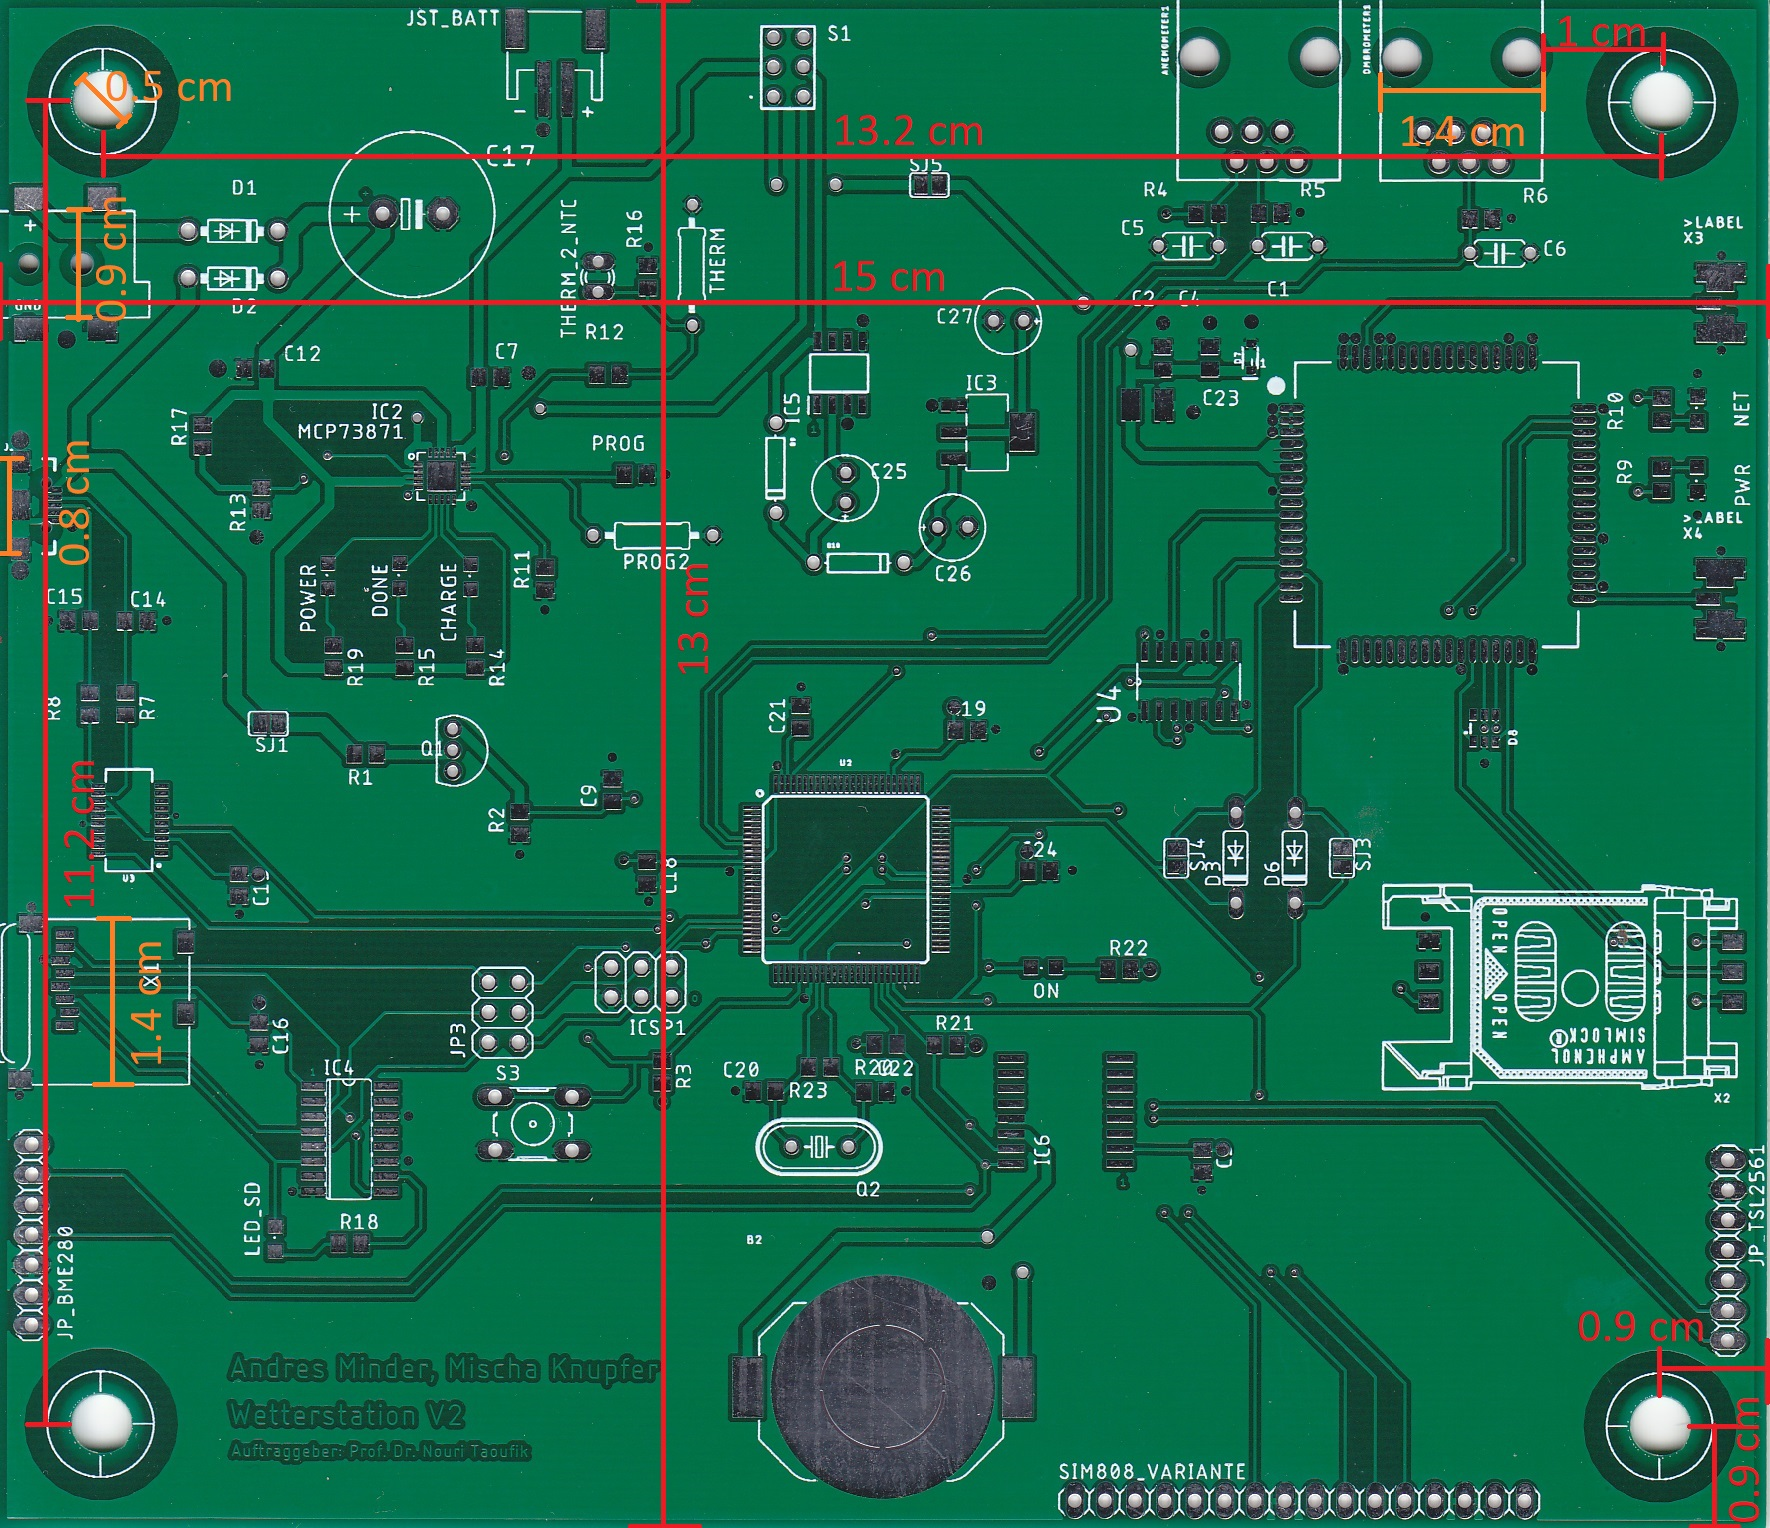
\includegraphics[width=0.9\linewidth]{graphics/Gehaeuse/PCB_Dimensionen.jpg}
\caption{Das noch unbestückte PCB mit den wichtigsten Dimensionen.}
\label{fig:Dimensionen1}
\end{figure}
\newpage
Abbildung \ref{fig:Dimensionen1} zeigt das noch unbestückte PCB, wie es schon in der Hardware Übersicht verwendet wurde, mit den wichtigsten Dimensionen. Das PCB hat eine Breite von 15cm, eine länge von 13cm. Die Mittelpunkte der 5mm breiten Bohrlöcher sind 13.2cm weit entfernt in der Breite und 11.2cm in der Länge, wobei diese jeweils 9mm vom Rand entfernt sind. Die Breite der Bauteile die aus dem Gehäuse hinausragen sind 1.4cm (RJ11, $\mu$SD), 0.9cm (DCIN Jack) und 0.8cm ($\mu$USB). Damit alle Bauteile von der Höhe her Platz haben, muss das Gehäuse nach oben hin mindestens über 3cm Freiraum verfügen wegen dem zum MCP73871 gehörenden Elektroly-Kondensator (C17). Der Akkumulator soll ebenfalls im Gehäuse Platz finden, weshalb genügend Platz (min. 2cm) in der Tiefe für diesen zur Verfügung stehen muss. Da es eine Bestückungsvariante gibt für den SIM808, soll das Gehäuse an der unteren Seite um mindestens 4cm erweitert werden, da das Breakout Board des SIM808 ansonsten nicht angeschlossen werden kann. Auf der rechten Seite werden Antennen für den SIM808 angeschlossen, weshalb das Gehäuse auf dieser Seite um mindestens 1cm erweitert werden soll, damit diese nicht knicken. Ebenfalls sollen auch die Kabel des Akkumulators vom knicken geschützt werden, hier benötigt man eine erweiterung des Gehäuses von mindestens 3mm, da die Kabel selbst eine höhere Flexibilität als die Antennen aufweisen. Auf der linken Seite befindet sich die $\mu$USB-Buchse, sowie die Öffnung für die $\mu$SD-Karte. Diese Öffnungen ragen ein wenig hinaus und sollten gut geschützt werden, weshalb eine Erweiterung der Dimensionierung auf der Linken Seite von 1mm empfohlen ist. Äusserst wichtig ist ebenfalls, dass der BME280 auf der linken Seite des Gehäuses nach aussen gebracht wird und in einem gut mit Aussenluft durchströmten eigenen Raum seinen Platz findet. Der TSL2561 wird ebenfalls auf der rechten Seite nach aussen geführt, damit dieser dort unter einem mit durchsichtigem Plexiglas versehenen eigenen Raum die Lichtintensität messen kann.\\[0.5cm]
Die wichtigsten Punkte wurden erläutert, weshalb es nun zum Design des Gehäuses kommt, welches im nächsten Abschnitt vorgestellt wird.

\subsubsection{Das Design}
Im vorhergehenden Unterkapitel wurden die wichtigsten Merkmale und Dimensionen des Gehäuses erläutert. In diesem Unterkapitel wird nun das provisorische Design vorgestellt. Da für den Zusammenbau das PCB auf einen Teil des Gehäuses gelegt wird und mit einem zweiten Teil überdeckt, wird in diesem Abschnitt der Begriff \textit{Boden} für den unteren Teil und \textit{Deckel} für den oberen Teil verwendet. Das Design wurde mit dem CAD-Programm Autodesk Fusion 360 erstellt, welches den Studenten von Bildungseinrichtungen wie der FHNW frei zur Verfügung steht.
\newpage

\begin{figure}[h]
\centering
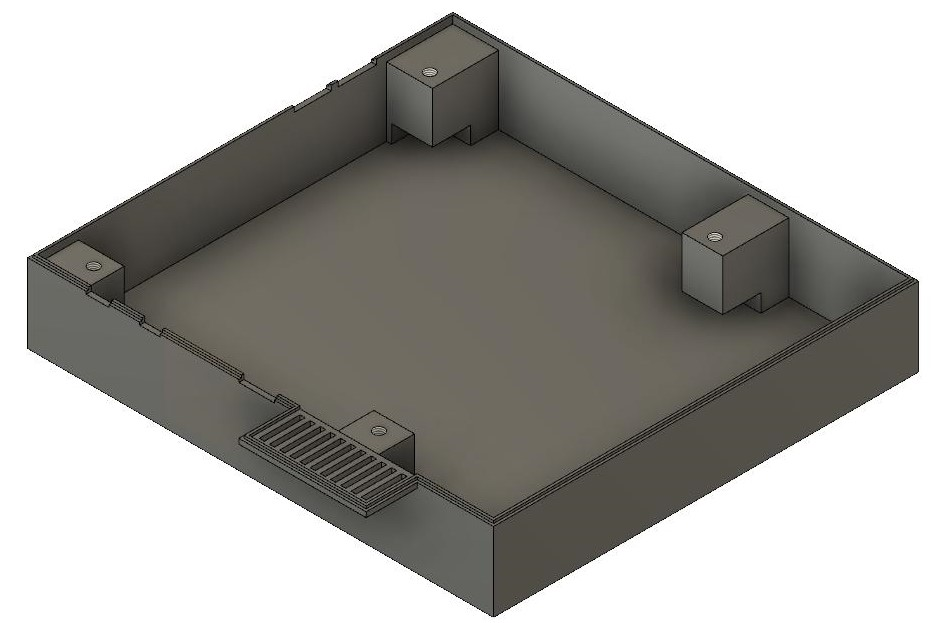
\includegraphics[width=0.99\linewidth]{graphics/Gehaeuse/Design_Boden.jpg}
\caption{Gesamtansicht des Designs des Bodens.}
\label{fig:D:Boden}
\end{figure}

Die Gesamtansicht des Designs des Bodens ist in Abbildung \ref{fig:D:Boden} zu sehen. Diverse Blöcke und Aussparungen sind deutlich zu sehen, worauf mit der Hilfe von den nachfolgenden Abbildungen näher eingegangen wird.\\

{\begin{minipage}[b][8cm][t]{0.39\textwidth}
Das PCB muss erhöht sein, damit der Akku darunter Platz findet. Ausserdem soll eine Schraube das Gehäuse mit dem PCB verbinden. Aus diesen Gründen wurden im Boden Blöcke implementiert, welche ein Schraubengewinde besitzen, wie in Abbildung \ref{fig:D:Boden:Schrauben} ersichtlich ist. Am unteren Ende des Schraubenblocks befindet sich eine Aussparung. Diese Aussparung bietet Platz für eine Mutter, falls das implementierte Gewinde fehlerhaft gedruckt wird.
\end{minipage}}
{\begin{minipage}[b][8cm][t]{0.6\textwidth}
\centering
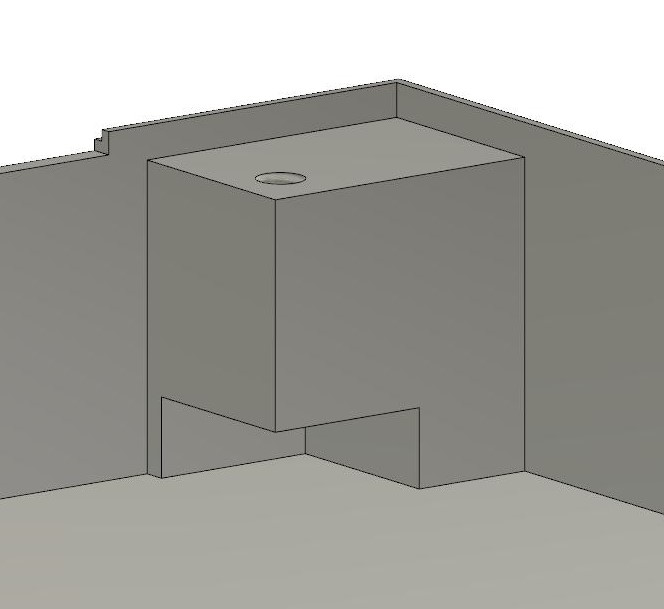
\includegraphics[width=0.8\linewidth]{graphics/Gehaeuse/Design_Boden_Schrauben.jpg}
\captionof{figure}{Design des Schraubenblocks des Bodens.}
\label{fig:D:Boden:Schrauben}
\end{minipage}}

\newpage
\begin{figure}[h]
\centering
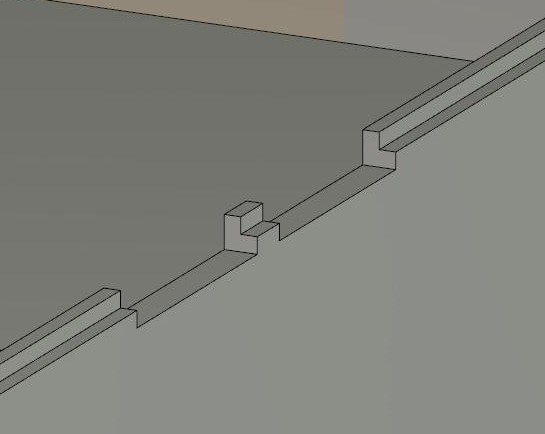
\includegraphics[width=0.5\linewidth]{graphics/Gehaeuse/Design_Boden_Aussparungen.jpg}
\caption{Aussparungen für Bauteile, welche aus dem Gehäuse hinausragen.}
\label{fig:D:Boden:Aussparungen}
\end{figure}
Die in Abbildung \ref{fig:D:Boden:Aussparungen} ersichtlichen Aussparungen sind notwendig um Öffnungen im Gehäuse zu generieren, welche Platz für die hinausragenden Bauteile bieten. Beim Boden sind diese Aussparungen alle gleich tief, da die Bauteile alle auf dem planen PCB angelötet sind und dieses somit als Referenz gilt.

\begin{figure}[h]
\centering
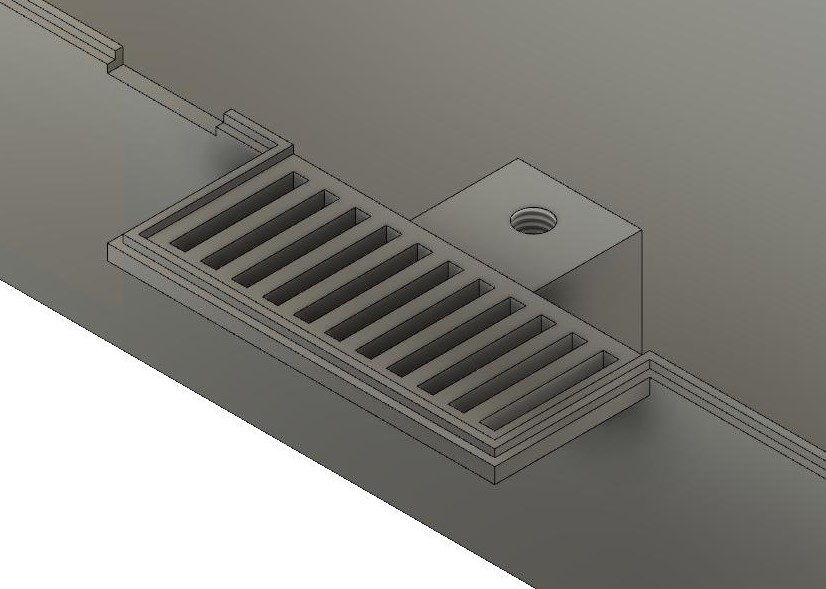
\includegraphics[width=0.7\linewidth]{graphics/Gehaeuse/Design_Boden_BME.jpg}
\caption{Seitenwand für den BME280-Extraraum mit Luftschlitzen.}
\label{fig:D:Boden:BME}
\end{figure}
Der BME280 muss nach aussen geführt werden in einen kleinen Extraraum, welcher gut belüftet ist. Nur so ist der BME280 in der Lage, die exakten Messwerte liefern zu können. Aus diesem Grund wird ein kleiner Extraraum am Rand des Gehäuses gefertigt, welcher mit Luftschlitzen versehen ist. In Abbildung \ref{fig:D:Boden:BME} sieht man den Boden für den im Deckel implementierten Extraraum. Der Boden ist, wie erwähnt, mit 2mm breiten Luftschlitzen versehen.

\newpage

\begin{figure}[h]
\centering
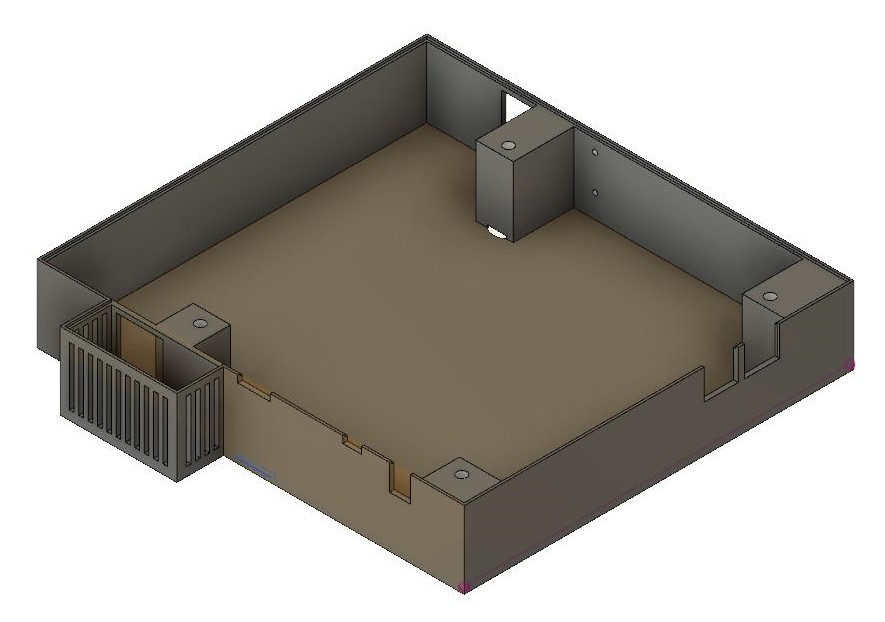
\includegraphics[width=0.99\linewidth]{graphics/Gehaeuse/Design_Deckel.jpg}
\caption{Gesamtansicht des Designs des Deckels.}
\label{fig:D:Deckel}
\end{figure}
Die Gesamtansicht des Designs des Deckels ist in Abbildung \ref{fig:D:Deckel} zu sehen. Wie schon beim Boden sind auch hier diverse Blöcke und Aussparungen zu sehen, auf welche mit der Hilfe von den nachfolgenden Abbildungen näher eingegangen wird.\\

{\begin{minipage}[b][9cm][t]{0.39\textwidth}
Die Schraubenblöcke des Deckels sind weniger interessant, da diese durchgehende Blöcke sind mit einem entsprechenden Gewinde. Aus diesem Grund wurde in Abbildung \ref{fig:D:Deckel:Schrauben} die Aussenseite des Deckels abgebildet, welche die Schraubenversenkung zeigt. In dieser Schraubenversenkung wird der Kopf der verwendeten Schraube seinen Platz finden, weshalb es zu keinem herausragen einer Schraube kommt.
\end{minipage}}
{\begin{minipage}[b][9cm][t]{0.6\textwidth}
\centering
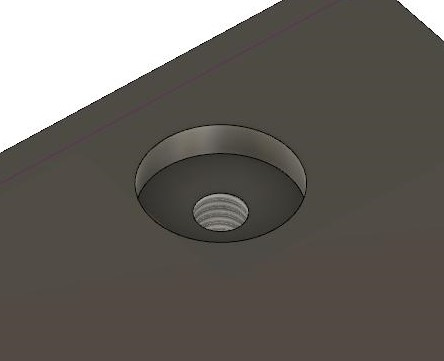
\includegraphics[width=0.8\linewidth]{graphics/Gehaeuse/Design_Deckel_Schraubenversenkung.jpg}
\captionof{figure}{Schraubenversenkung im Deckel.}
\label{fig:D:Deckel:Schrauben}
\end{minipage}

\begin{figure}[h]
\centering
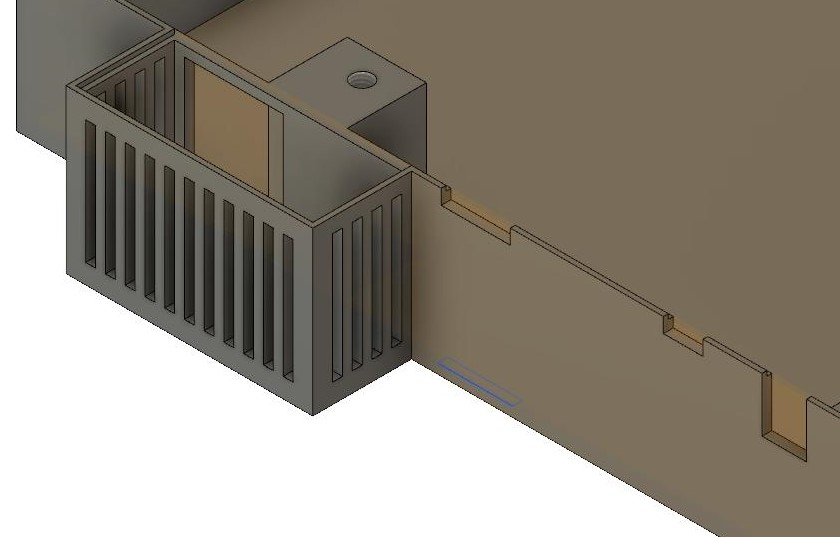
\includegraphics[width=0.6\linewidth]{graphics/Gehaeuse/Design_Deckel_BMEundAussparungen.jpg}
\caption{Aussparungen für Bauteile, welche aus dem Gehäuse hinausragen und der designte Extraraum für den BME280 mit Luftschlitzen.}
\label{fig:D:Deckel:BME}
\end{figure}
Abbildung \ref{fig:D:Deckel:BME} zeigt den bereits erwähnten Extraraum des BME280. Die Luftschlitze sind deutlich zu erkennen und an jeder Seite des Extraraumes angebracht. Ausserdem ist auf dieser Abbildung ebenso ersichtlich, dass die Aussparungen verschiedene Höhen aufweisen. Die Höhe einer Aussparung ist Bauteilabhängig, genauso wie deren Breite.

\begin{figure}[h]
\centering
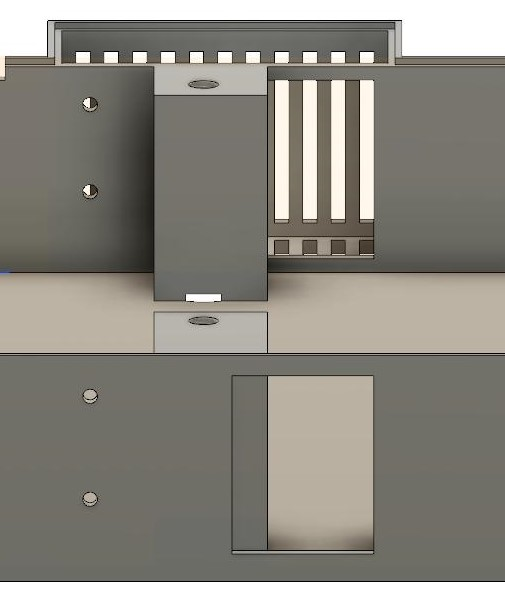
\includegraphics[width=0.5\linewidth]{graphics/Gehaeuse/Design_Deckel_TSL.jpg}
\caption{Öffnung und Bohrungen für den TSL2561 und den BME280.}
\label{fig:D:Deckel:TSL}
\end{figure}
Um den BME280 und den TSL2561 hinausführen zu können, wurden im Gehäuse entsprechende Öffnungen und auch Schraubenlöcher eingelassen. Die eben genannten Öffnungen und Schraubenlöcher sind in Abbildung \ref{fig:D:Deckel:TSL} äusserst gut ersichtlich.
\newpage
{\begin{minipage}[b][7cm][t]{0.49\textwidth}
\centering
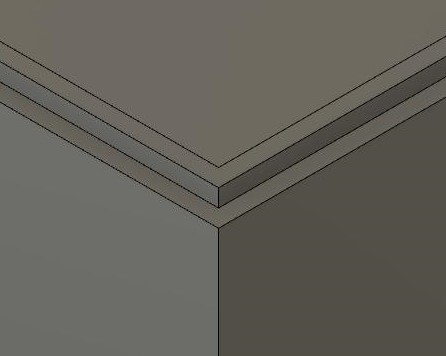
\includegraphics[width=0.8\linewidth]{graphics/Gehaeuse/Design_Boden_Rand.jpg}
\captionof{figure}{Design des Randes vom Boden zum Deckel hin.}
\label{fig:D:Boden:Rand}
\end{minipage}}
{\begin{minipage}[b][7cm][t]{0.49\textwidth}
\centering
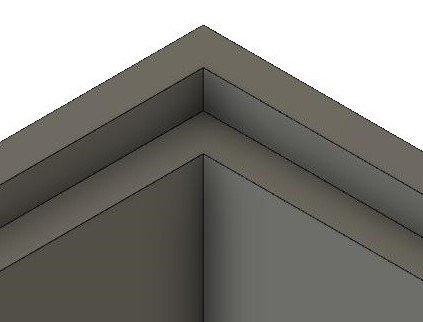
\includegraphics[width=0.8\linewidth]{graphics/Gehaeuse/Design_Deckel_Rand.jpg}
\captionof{figure}{Design des Randes vom Deckel zum Boden hin.}
\label{fig:D:Deckel:Rand}
\end{minipage}}

Damit das Befestigen des Bodens mit dem Deckel einfacher zu handhaben ist, wurde beim Boden die äussere Hälfte des Randes um 1mm gesenkt, wobei beim Deckel die innere Hälfte des Randes um 1mm gesenkt wurde. Dank diesem Feature ist es möglich den Deckel wie ein Puzzlestück am Boden anzubringen, bevor die Verschraubung von statten geht.\\[0.5cm]
Das Design des Gehäuses für das PCB wurde in diesem Unterkapitel näher erläutert. Es sei jedoch erwähnt, dass dieses Gehäuse nicht geeignet ist um die Wetterstation im freien betreiben zu können. Das hier vorgestellte Design zeigt lediglich auf, auf was beim Gehäuse, in Bezug auf das PCB, geachtet werden muss. Damit das Gehäuse für den Gebrauch im freien taugt, muss es zwingend gegen Regen und Staub dicht sein, so dass die verwendete Elektronik keine Schäden erleidet. Dennoch muss der BME280 mit Aussenluft belüftet werden, was bei einem möglichst Regen- und Staubdichten Gehäuse eine zusätzliche, kontrollierte Belüftung notwendig macht. Ausserdem muss auf einen möglichen Hitzestau durch Sonneneinstrahlung getestet und gegebenfalls eine Kühlung integriert werden.


\part{Abschluss}
\label{part:AbschliessenderTeil}
\chapter{Konzeptvalidierung}
\label{chap:Konzeptvalidierung}
\chapter{Schluss}
\label{chap:Schluss}

\newpage


\chapter{Authentizitätserklärung}

Wir, Mischa Knupfer und Andres Minder, versichern, dass dieses Projekt und Fachbericht selbstständig erarbeitet wurden. Alle Quellen und Hilfsmittel aus anderen Werken, die dem Wortlaut oder dem Sinne nach entnommen wurden und zu dieser Arbeit beigetragen haben, sind jeweils kenntlich referenziert.\\

Aufgrund dessen, dass der Fachbericht als PDF per E-Mail abgegeben wurde, wie vom Auftraggeber/Betreuer gefordert, wird keine Unterschrift gesetzt. \\
\vfill
\begin{center}
\begin{tabular}{p{5cm}p{1cm}l}
\Large\textbf{Ort, Datum:} & & \Large\textbf{Mitwirkende:} \\
\vspace{1cm} & \vspace{1cm} & \vspace{1cm} \\
\Large{Brugg/Windisch, \today} & & \\
\end{tabular}
\end{center}
%%---BIBLIOGRAPHY------------------------------------------------------------------------
\part{Referenzen}
{\sloppypar
\printbibliography[heading=bibintoc]
\label{sec:lit}
%\selectlanguage{english}				%ngerman or english
%\printbibliography[heading=bibintoc]
}

\listoftables
\listoffigures
%%---APPENDIX----------------------------------------------------------------------------
\begin{appendix}



\end{appendix}



%%---NOTES for DEBUG---------------------------------------------------------------------
\ifdraft{%Do this only if mode=draft
%%requires \usepackage{todonotes})
\newpage
\listoftodos[\section{Todo-Notes}]
\clearpage
}
{%Do this only if mode=final
}
\end{document}
